\chapter{能量与轨道角动量}

PINEM 的能量谱只记录电子与光场交换的净能量，并不总能辨认完成交换的量子路径。如果两次 $\omega$ 交换与一次 $2\omega$ 交换都给出 $2\hbar\omega$，能量探测器便把它们归入同一通道；当两束光还携带不同的轨道角动量（OAM）时，联合测量可能重新区分这两条历史。设每次 $\omega$ 与 $2\omega$ 交换分别转移 $\ell_1\hbar$、$\ell_2\hbar$，那么 $2\ell_1\ne\ell_2$ 时终态不同，而 $2\ell_1=\ell_2$ 时两条历史仍可在同一终态干涉。OAM 因而既是额外的观测坐标，也能成为控制相干路径可区分性的工具。

要描述后者，只需先把能量和 OAM 作为离散量子数，而不必预设二维实体晶格。只有多个交换过程在这些坐标上构成可重复的平移，Bloch 准动量与合成晶格能带的语言才适用；一旦不同路径落到同一终态，则须对振幅求和，而不能把路径概率简单相加。


用 $n$ 表示能量交换阶数，用 $\ell$ 表示电子轨道角动量量子数（$L_z=\ell\hbar$），用 $m$ 表示光学涡旋或等离激元的拓扑荷。$(n,\ell)$ 是单电子模空间中的合成坐标，不是实空间晶格坐标。只有在给定有效哈密顿量、能隙和边界条件后，Berry 曲率、Chern 数、Wilson 环或非厄米绕数才具有各自严格的拓扑含义。


\section{能量–OAM 跃迁}
近场的角向 Fourier 因子给出这些离散平移的选择规则。考虑一个带有方位相位的模式。若场的相关分量含有 $\ee^{\ii m\phi-i\omega t}$，吸收一个该模式量子时电子除了获得能量 $\hbar\omega$，还获得轨道角动量 $m\hbar$。用 $|n,\ell\rangle$ 表示相对中心能量交换了 $n$ 个光子、轨道角动量为 $\ell\hbar$ 的电子态，则单一模式产生的基本跃迁满足

\begin{equation}
|n,\ell\rangle\longrightarrow |n+1,\ell+m\rangle .
\label{eq:ch03-1}
\end{equation}

式~\cref{eq:ch03-1} 同时规定了两种守恒荷的改变：电子能量增加一个光量子，绕束轴的角动量增加 $m\hbar$。交换 $j$ 个光量子时，角相位随之乘成 $\ee^{\ii jm\phi}$，所以选择规则变为 $\Delta n=j,\Delta\ell=jm$。这个结果可以直接从散射波函数在角动量基底中的 Fourier 系数检验，并不要求预先假设合成晶格。待多个驱动模式出现，再把各自的交换向量放在同一个整数格点中考虑。


单个涡旋场先给出最基本的选择规则。Cai 等\textsuperscript{\hyperref[ch03-ref1]{[1]}}从手性等离激元的纵向近场得到交换 $j$ 个光量子后的幅度
\[
f_j(R,\varphi)=\ii^j\ee^{\ii jm\varphi}J_j\!\left[2\eta J_m(k_pR)\right],
\qquad \eta=\frac{2g\Omega}{1+\Omega^2}.
\]
角因子说明电子获得 $jm\hbar$ 的 OAM，径向贝塞尔因子决定各通道出现的几率，$\eta$ 在 $\Omega=1$ 时达到最大。因而提高近场绕数 $m$ 可以在有限交换阶数下获得较大的输出 OAM，而无需假定电子吸收非常多的光量子。电子态的方位电流也可由这个角相位直接计算，并非单纯的绘图标签。

\begin{figure}[!htbp]
\centering
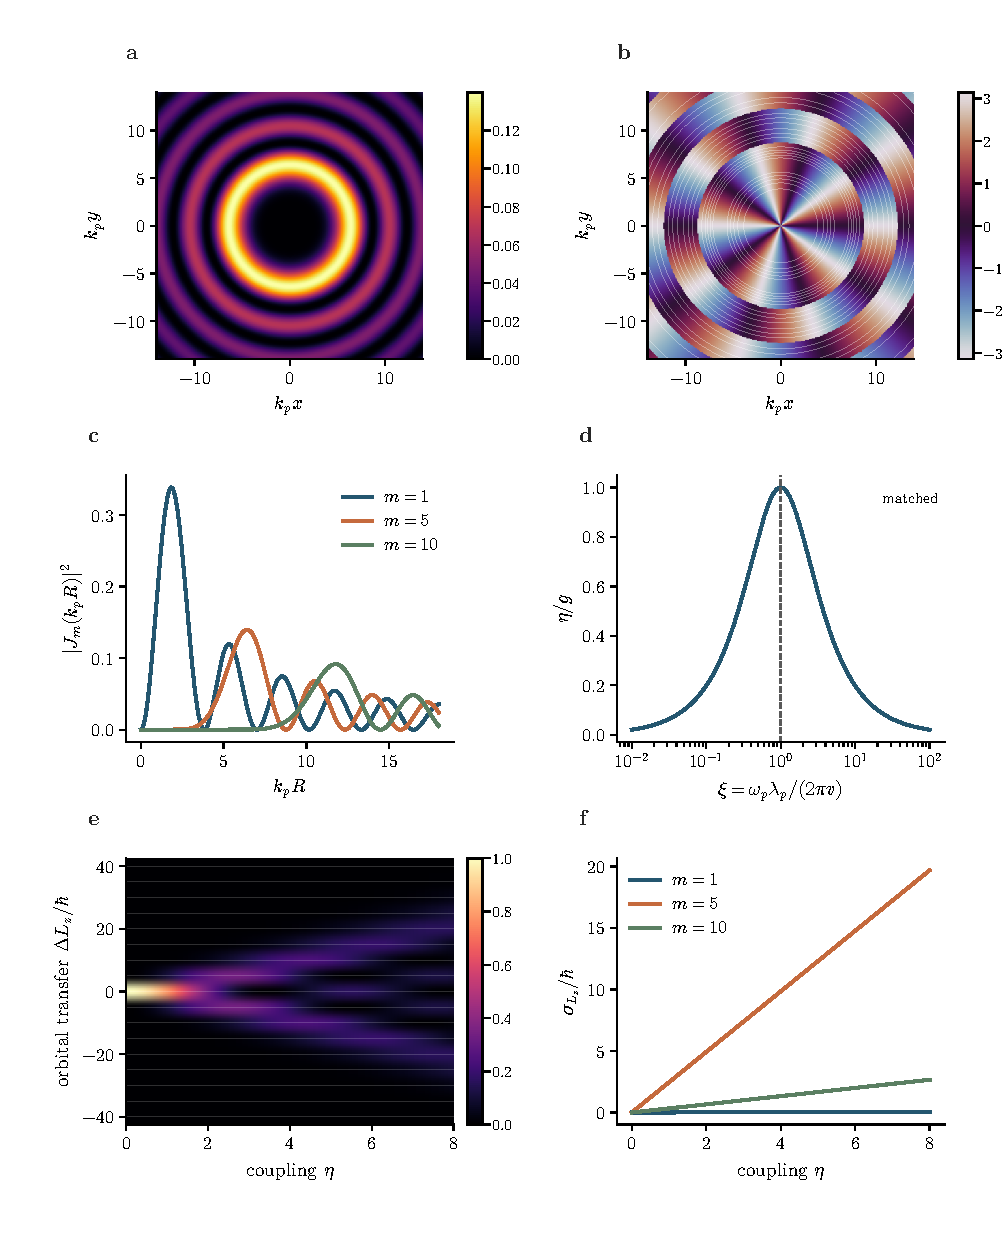
\includegraphics[width=0.96\linewidth,height=0.70\textheight,keepaspectratio]{cai2018_oam_transfer.pdf}
\caption{\textbf{等离激元向电子转移轨道角动量}\quad 这组图把 OAM 转移的整条物理链条连了起来。上排先画出手性表面等离激元的近场纹理：强度图给出环形耦合区域，位相图显示 $m$ 重绕行，而径向 $J_m(k_pR)$ 包络决定不同半径处的局域耦合强弱。左下再给出速度匹配效率，说明为什么只有接近相位匹配时这些通道才会真正显现。右下两图则把选择规则转换成可观测结果：联合通道图显示每发生一步能量交换，就固定伴随 $m\hbar$ 的轨道角动量转移；带宽图进一步说明高拓扑荷模式会显著放大输出 OAM 梯子的宽度。这样，近场纹理、选择规则与最终电子边带不再是分散的示意，而是同一过程的连续读出。}
\label{fig:ch03-theory-atlas--10-cai2018-oam-transfer}
\end{figure}

具体到各面板，(a,b) 在 $k_px,k_py\in[-14,14]$ 的 $320^2$ 网格上计算 $E_z\propto J_5(k_pR)\ee^{\ii5\varphi}$ 的强度和相位主值；相位在 $|J_5|=0$ 处没有物理可观测定义。(c) 对 $m=1,5,10$ 求 $|J_m(k_pR)|^2$，其中 $k_pR\in[0,18]$、共 600 点。(d) 使用 $\xi\in[10^{-2},10^2]$ 的 450 点扫描绘出 $\eta/g=2\xi/(1+\xi^2)$；这只是归一化的速度匹配代理，不能替代具体场模式的 Maxwell 轨迹积分。(e) 固定 $m=5,k_pR_0=7$，画 $P_n(\eta)=J_n^2[2\eta|J_5(7)|]$，$|n|\le8$，并把每阶映到 $\Delta L_z=n m\hbar$；耦合 $\eta\in[0,8]$ 取 280 点。(f) 对 $m=1,5,10$ 与相同 $R_0=7$，以 $|n|\le18$ 计算 $\sigma_{L_z}/\hbar=[\sum_n(nm)^2P_n]^{1/2}$，$\eta\in[0,8]$ 取 240 点。这里的 $m$ 为近场方位绕数，而不是未经标定的实验绝对 OAM。


要把上述选择规则变成实验观测，必须分辨能量与 OAM 两个坐标。Tavabi 等\textsuperscript{\hyperref[ch03-ref2]{[2]}}使用 OAM 分析读出非弹性散射后的 $I(E,\ell)$；当激发具有空间离域性或电子束偏离轴线时，不同整数角动量分量会混合。因此二维原始计数与通过仪器响应模型解混得到的 OAM 通道权重不完全相同。这里所称的额外信息坐标并非理想无噪声的数学标签，而必须与排序器串扰同时建模。

当至少两种线性无关的跃迁向量同时存在，能量与 OAM 不能再用一条一维链表示。二维合成晶格的优势在于：不同光学模式的幅度直接变成跃迁强度，相对相位直接变成 Peierls 相位，因此实验旋钮与紧束缚参数一一对应。下面的色散、波包传播和等能线图都由同一个离散哈密顿量产生。

若同时存在 $\omega$ 与 $2\omega$ 两色交换，则一个能量阶可能由多个不同整数事件数 $(n_1,n_2)$ 实现。Li 等\textsuperscript{\hyperref[ch03-ref3]{[3]}}证明给两种驱动设置适当的 OAM 荷，可以用第二坐标解除这种简并并构造二维合成晶格；他们还利用耦合比改变等能线连通性。理解这些结果的关键不是先画能带，而是求清楚整数交换数到可测 $(N,\ell)$ 的映射，以及在什么条件下该映射可逆。下面沿这一映射推导输出振幅与有效色散。

设两束光的频率为 $\omega$ 与 $2\omega$，各自对应互相可交换的升阶算符 $T_j$，并取 $\beta_j=|\beta_j|\ee^{\ii\vartheta_j}$。在无反冲近似下，$U=U_1U_2$ 且 $U_j=\exp(-\beta_jT_j+\beta_j^*T_j^\dagger)$。由 Jacobi--Anger 展开得
\begin{equation}
U_j=\sum_{n_j=-\infty}^{\infty}J_{n_j}(2|\beta_j|)\ee^{\ii n_j\arg(-\beta_j)}\,T_j^{n_j},
\end{equation}
其中 $T_j$ 把电子能量平移 $\hbar\omega_j$，若该光场携带 OAM 荷 $\ell_j$，还同时把电子 OAM 平移 $\ell_j\hbar$。于是隐藏的光子交换格点 $(n_1,n_2)$ 上振幅严格因子化为
\begin{equation}
c_{n_1n_2}=\prod_{j=1}^{2}J_{n_j}(2|\beta_j|)\ee^{\ii n_j\arg(-\beta_j)}.
\label{eq:ch03-li-coeff}
\end{equation}

标准 EELS 只测总能量。对 $\omega_2=2\omega_1=2\omega$，所有满足 $N=n_1+2n_2$ 的路径都落在同一能量边带。若只保留能量坐标，最终振幅是沿这条整数直线的相干和，二维交换历史就发生“谱坍缩”。引入 OAM 后，第二个观测坐标为
\begin{equation}
\begin{pmatrix}N\\ \ell\end{pmatrix}
=\underbrace{\begin{pmatrix}1&2\\ \ell_1&\ell_2\end{pmatrix}}_{A}
\begin{pmatrix}n_1\\n_2\end{pmatrix}.
\label{eq:ch03-li-map}
\end{equation}
将行列式记为 $D=\ell_2-2\ell_1$。当 $D\neq0$，矩阵逆给出每个候选末态的唯一事件数，
\begin{equation}
 n_1=\frac{\ell_2N-2\ell}{D},\qquad
 n_2=\frac{\ell-\ell_1N}{D}.
 \label{eq:oam-integer-inverse}
\end{equation}
事件数必须是整数，因此这两个分式为整数是实际可达性的必要且充分条件。例如 $\ell_1=\ell_2=-1$ 时 $D=1$，每个整数 $(N,\ell)$ 都对应唯一的 $(n_1,n_2)$；若 $|D|>1$，可达末态只构成 $\ZZ^2$ 的一个指数为 $|D|$ 的子格。这一指数来自整数矩阵在单位元胞上的有向面积 $|\det A|$，并不能仅由实数上的可逆性推出。

当 $D=0$，矩阵存在整数核向量 $(-2,1)$。如果 $(n_1^{(0)},n_2^{(0)})$ 是某一末态的解，那么全部可能的交换历史是
\begin{equation}
 (n_1,n_2)=(n_1^{(0)}-2k,\,n_2^{(0)}+k),\qquad k\in\ZZ.
 \label{eq:oam-degenerate-histories}
\end{equation}
对这些历史必须先相干求和，之后才能取概率：
\begin{equation}
 C_{N\ell}=\sum_{k\in\ZZ}c_{n_1^{(0)}-2k,\,n_2^{(0)}+k},\qquad
 P_{N\ell}=|C_{N\ell}|^2.
 \label{eq:oam-degenerate-amplitude}
\end{equation}
这说明 OAM 坐标何时真正解除了历史简并，也指出有限探测分辨率和物理上不同的未观测末态会在哪里重新改变相干求和规则。


两个最小交换事件 $(1,0)$ 和 $(0,1)$ 在可观测平面中变成
\begin{equation}
\vb v_1=(1,\ell_1),\qquad \vb v_2=(2,\ell_2).
\end{equation}
将 $|N,\ell\rangle$ 记为格点 $|\vb R\rangle$。为把幺正相位调制写成厄米紧束缚生成元，定义复跳跃矩阵元 $t_j=-\ii\beta_j=|\beta_j|\ee^{\ii\phi_j}$，即 $\phi_j=\vartheta_j-\pi/2$。因此这里的 $\phi_j$ 是哈密顿量跳跃相位，与近场耦合章节定义的 $\arg\beta_j$ 相差固定的 $\pi/2$；二者不能在相干振幅中直接混用。无量纲生成元为
\begin{equation}
H_{\rm eff}=\sum_{\vb R}\left(
t_{\omega}|\vb R+\vb v_1\rangle\langle\vb R|
+t_{2\omega}|\vb R+\vb v_2\rangle\langle\vb R|+\text{H.c.}\right),
\label{eq:ch03-li-heff}
\end{equation}
并满足 $U=\exp(-\ii H_{\rm eff})$。因此高阶边带并不是额外加入的长程跃迁；它们是最近邻生成元经过有限“演化时间”后由多步路径自然产生的。这个区分非常重要，因为以后若要加入无序、损耗或合成磁通，应该修改生成元，而不是直接修改最终贝塞尔人口。

采用 Bloch 约定 $|\vb K\rangle\propto\sum_{\vb R}\ee^{-\ii\vb K\cdot\vb R}|\vb R\rangle$，升阶算符的本征值为 $\ee^{\ii\vb K\cdot\vb v_j}$。因此\cref{eq:ch03-li-heff} 给出
\begin{equation}
\varepsilon(\vb K)=2|\beta_\omega|\cos(\vb K\cdot\vb v_1+\phi_\omega)
+2|\beta_{2\omega}|\cos(\vb K\cdot\vb v_2+\phi_{2\omega}).
\label{eq:ch03-li-band}
\end{equation}
对论文使用的共旋情形 $\ell_1=\ell_2=-1$，两个相位在无限、无缺陷 Bravais 晶格上可由晶格规范变换吸收，因此 Lifshitz 重连由幅度比而不是绝对光学相位控制。令 $q_j=\vb K\cdot\vb v_j+\phi_j$，鞍点满足 $\sin q_1=\sin q_2=0$；零准能又要求
\begin{equation}
|\beta_\omega|\cos q_1+|\beta_{2\omega}|\cos q_2=0.
\end{equation}
在两个余弦异号的鞍点，这立刻给出
\begin{equation}
\eta_c\equiv\frac{|\beta_{2\omega}|}{|\beta_\omega|}=1.
\label{eq:ch03-li-critical}
\end{equation}
所以论文中的临界比值不是从数值图“看出来”的，而是零准能曲线穿过鞍点的解析条件。态密度
\begin{equation}
\rho(\varepsilon)=\frac{1}{(2\pi)^2}\int_{\rm BZ}\dd ^2K\,\delta[\varepsilon-\varepsilon(\vb K)]
\end{equation}
在二维鞍点附近出现范霍夫增强，这才把几何重连与可计算谱特征连接起来。

\begin{figure}[!htbp]
\centering
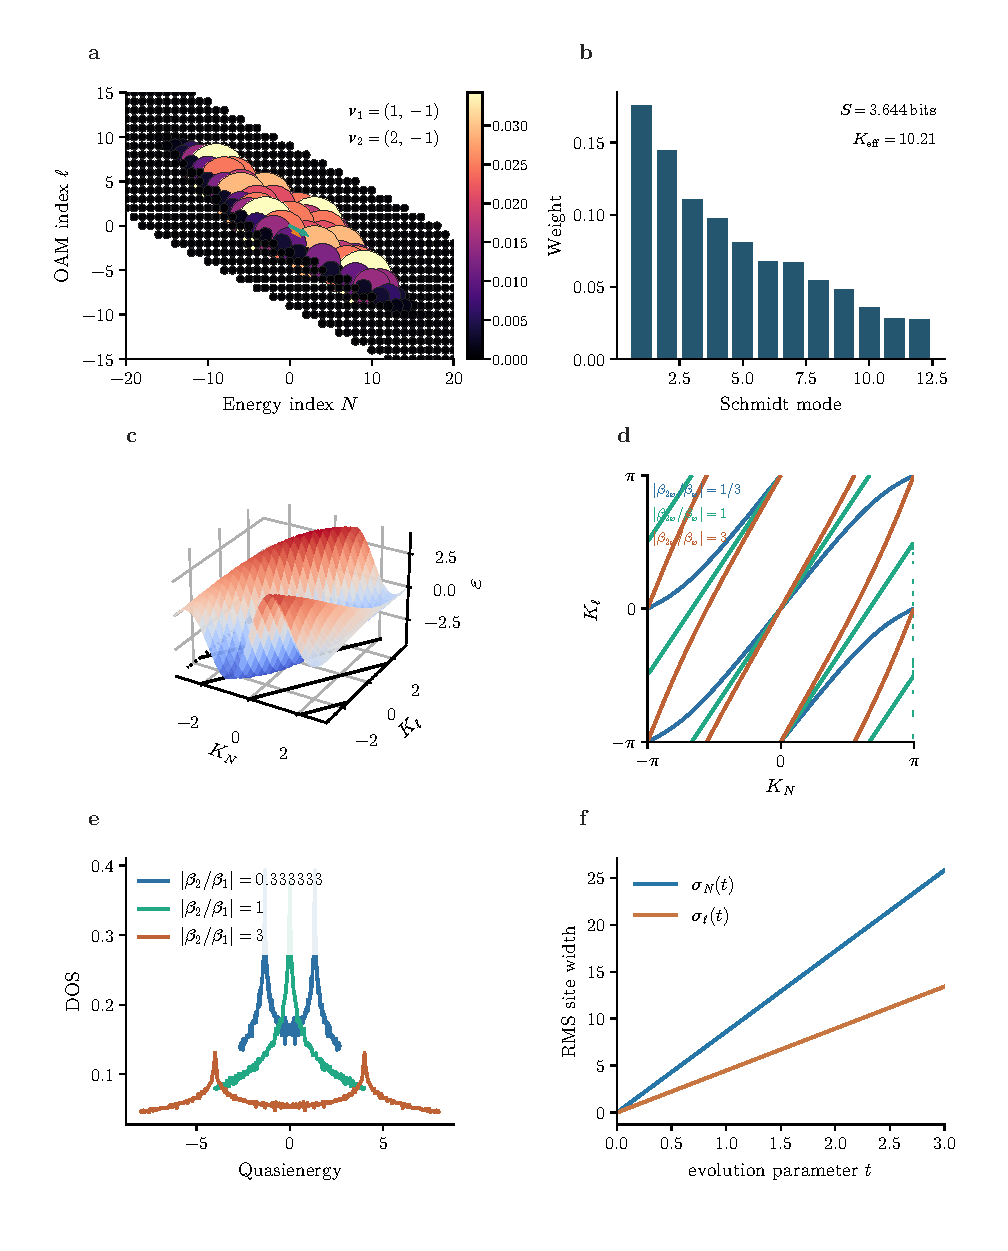
\includegraphics[width=0.96\linewidth,height=0.70\textheight,keepaspectratio]{li2026_synthetic_lattice_unified.pdf}
\caption{\textbf{二维能量--OAM 合成晶格}\quad (a) 由两种携带轨道角动量的光子交换构成的真实二维可达格点及联合概率；(b) 能量--OAM 模态系数矩阵的奇异值权重谱；(c) 双频合成准能带的三维色散面；(d) 改变两色耦合比时零准能等值线的 Lifshitz 重连；(e) 同一色散下的态密度峰；(f) 在固定耦合比下，量子行走波包沿能量轴和 OAM 轴的均方根宽度随传播参数增长，直接量化各方向的输运速度。这六种诊断区分了概率结构、模态分解、谱几何和传播动力学；其中模态不可分性不能直接解释为两个电子间的纠缠。}
\label{fig:ch03-theory-atlas--13-li2026-synthetic-lattice-unified}
\end{figure}

具体到各面板，(a) 用两个驱动强度 $|\beta_1|=|\beta_2|=2$，对交换阶截断 $|n_j|\le18$ 计算联合概率，再映射到 $N=n_1+2n_2,L=-n_1-n_2$ 并按概率大小绘制真实可达晶格点。(b) 对同一能量--OAM 振幅矩阵取奇异值谱，显示前 12 个权重；该量表示所选模式分解下的不可分性，不直接等于两电子纠缠。(c) 在 $180^2$ 准动量格点取 $|\beta_1|=|\beta_2|=1$ 画 $\varepsilon(K_N,K_L)$ 三维面。(d) 对强度比 $1/3,1,3$ 计算同一准能带的零能等值线。(e) 分别用 $360^2$ 格点与 250 个直方箱估计三组参数的态密度；峰位和峰高有有限网格、箱宽误差。(f) 取 $|\beta_1|=1,|\beta_2|=3$ 和 $120^2$ 准动量格点，将单点初态按 $\psi_{N\ell}(t)=\operatorname{FFT}^{-1}[\ee^{-\ii\varepsilon(\vb K)t}]$ 演化，在 $t\in[0,3]$ 的 91 个时刻计算 $\sigma_N(t)=\sqrt{\langle N^2\rangle-\langle N\rangle^2}$ 及 $\sigma_\ell(t)=\sqrt{\langle\ell^2\rangle-\langle\ell\rangle^2}$。两条曲线反映不同方向的输运展宽，不将有限时间、有限格点的宽度增长称为严格的动力学相变。

这两条曲线还可以从平移代数直接求出，而不必依赖傅里叶网格。令 $X_a$ 为合成位置算符，$a=N,\ell$，若 $T_j|\vb R\rangle=|\vb R+\vb g_j\rangle$，则
\[
 [X_a,T_j]=g_{j,a}T_j,\qquad H_{\rm eff}=\sum_{j=1}^2(t_jT_j+t_j^*T_j^\dagger).
\]
因为这些无穷晶格上的平移算符彼此对易，$[H_{\rm eff},[H_{\rm eff},X_a]]=0$。对无量纲演化 $U(t)=\ee^{-\ii t H_{\rm eff}}$，海森堡算符的展开恰好在一阶终止：
\begin{align*}
 X_a(t)&=U(t)^\dagger X_aU(t)
 =X_a+\ii t[H_{\rm eff},X_a]\\
 &=X_a-\ii t\sum_j g_{j,a}(t_jT_j-t_j^*T_j^\dagger).
\end{align*}
单点初态 $|\vb R=\vb0\rangle$ 与相异跃迁后的格点态正交，因而 $\langle X_a(t)\rangle=0$，只有同一跃迁与其逆跃迁的模方进入二阶矩，得到
\begin{equation}
 \sigma_a^2(t)=\langle X_a(t)^2\rangle=2t^2\sum_{j=1}^2|t_j|^2g_{j,a}^2.
 \label{eq:li-ballistic-width}
\end{equation}
图中 $\vb g_1=(1,-1)$、$\vb g_2=(2,-1)$、$|t_1|=1$、$|t_2|=3$，故 $\sigma_N^2=74t^2$、$\sigma_\ell^2=20t^2$。有限 $120\times120$ 傅里叶网格在所示时间窗口内逼近这一无限晶格精确结果；图的纵向差异正是两种跃迁在能量、OAM 两坐标上的步长不同造成的。


这一推导也指出了几个真正值得继续做的问题。若引入第三个独立跳跃方向，光学相位不再必然全部是规范自由度，闭合回路上的相位和才可能形成不可消去的合成磁通；若引入位置依赖损耗，$H_{\rm eff}$ 变为非厄米，布里渊区能带与开边界谱可能不再等价；若实验只测有限 OAM 窗口，边界本身会改变量子行走。后面的拓展图只有在这些新增项被明确写进生成元以后，才可以被解释为对 Li 2026 模型的真正延伸。


\section{角相位同距性}
仅仅测出二维晶格里有哪些能量--OAM 末态，并不能保证能够反演产生它们的光学近场。原因是探测器直接给出概率模方，却没有记录每条振幅路径的复相位。这个困难在一个比完整 Maxwell 求解更简单的角向模型中就会出现。考虑入射 OAM 为零、沿角度均匀分布的电子，设其受到的经典 PINEM 轨迹耦合为
\begin{equation}
 \beta(\varphi)=a\,s(\varphi),\qquad a>0,\qquad |s(\varphi)|=1,
 \quad s(\varphi)=\ee^{\ii\chi(\varphi)}.
 \label{eq:oam-phase-only-coupling}
\end{equation}
这里 $a$ 是无量纲耦合强度，$\varphi$ 是电子横向位置的方位角，$\chi$ 是近场沿电子路径积累的相位。式中假设幅度与 $\varphi$ 无关，只研究相位所携带的信息；实际粒子附近的径向强度和角向幅度不一定满足这个假设。先前建立的贝塞尔展开给出第 $n$ 个能量边带的角波函数
\begin{equation}
 \psi_n(\varphi)=\frac{J_n(2a)}{\sqrt{2\pi}}
 \ee^{\ii n\arg[-\beta(\varphi)]}
 =\frac{(-1)^nJ_n(2a)}{\sqrt{2\pi}}s(\varphi)^n.
 \label{eq:oam-phase-only-sideband}
\end{equation}
这里的整体 $(-1)^n$ 不影响下述概率，却应在需要与其他散射路径相干叠加时保留。为了知道能量边带中的角结构，需要把 $\psi_n$ 投影到 $\ee^{\ii M\varphi}/\sqrt{2\pi}$ 这一归一化 OAM 基底。令
\begin{equation}
 c_{nM}=\int_0^{2\pi}\frac{\dd\varphi}{\sqrt{2\pi}}
 \ee^{-\ii M\varphi}\psi_n(\varphi)
 =(-1)^nJ_n(2a)\,\widetilde{s^n}_M,
 \qquad
 \widetilde{s^n}_M=\frac{1}{2\pi}\int_0^{2\pi}
 s(\varphi)^n\ee^{-\ii M\varphi}\,\dd\varphi.
 \label{eq:oam-phase-power-fourier}
\end{equation}
因而联合测量的概率及其按能量条件化的分布分别为
\begin{equation}
 P_{nM}=J_n^2(2a)|\widetilde{s^n}_M|^2,
 \qquad P(M\mid n)=|\widetilde{s^n}_M|^2.
 \label{eq:oam-homometry-joint}
\end{equation}
右边第二式成立的条件是对应能量边带确实有非零概率，且 OAM 收集窗口包含所有模。由 $|s|=1$ 与圆周 Fourier 基底完备性，
\begin{equation*}
 \sum_{M\in\mathbb Z}|\widetilde{s^n}_M|^2
 =\frac{1}{2\pi}\int_0^{2\pi}|s(\varphi)^n|^2\,\dd\varphi=1,
 \qquad
 \sum_M P_{nM}=J_n^2(2a).
\end{equation*}
这揭示了仅测能量时的一个严格盲区：所有具有同样常数模 $a$、但具有任意不同角相位 $\chi(\varphi)$ 的场，都会产生\emph{完全相同}的纯能量谱。即使进一步测量一个光子边带的 OAM，也不一定能够解除简并，因为不同函数可以拥有相同的 Fourier 模方，这称为角同距性。

这种简并为何会被高阶光子交换解除，可以直接从 Fourier 自相关恒等式看出来。把 $P(M\mid n)$ 沿 $M$ 作逆离散 Fourier 求和，代入\cref{eq:oam-phase-power-fourier} 并使用周期 delta 核，得到
\begin{align*}
 \sum_M P(M\mid n)\ee^{\ii M\Delta}
 &=\frac{1}{(2\pi)^2}\int\dd\varphi\,\dd\varphi'
 s(\varphi)^n s(\varphi')^{-n}
 \sum_M\ee^{\ii M(\Delta-\varphi+\varphi')}\\
 &=\frac{1}{2\pi}\int_0^{2\pi}
 \ee^{\ii n[\chi(\varphi+\Delta)-\chi(\varphi)]}\,\dd\varphi.
\end{align*}
因此第 $n$ 个边带测量的是\emph{角相位差的第 $n$ 阶圆矩}，不是把第一阶 OAM 谱简单放大 $n$ 倍。只要两种角场的第一阶圆矩相同而第二阶不同，单光子 OAM 就会同距，双光子 OAM 则可以将它们区分。

一个不需要拟合参数的精确构造来自六个等宽方位扇区。令每个扇区宽 $\Delta\varphi=\pi/3$，从 $j=0$ 起依次取两组相位因子
\begin{equation}
 A=(1,1,1,1,1,-1),\qquad
 B=(1,1,\ii,1,1,-\ii).
 \label{eq:oam-six-sector-masks}
\end{equation}
对整数 $M$，直接积分每个扇区而不作像素插值，有
\begin{equation}
 \widetilde{s^n}_M=
 \frac{\operatorname{sinc}(M\pi/6)}{6}
 \sum_{j=0}^{5}s_j^n\,
 \ee^{-\ii M(2j+1)\pi/6},
 \qquad \operatorname{sinc}x=\frac{\sin x}{x}.
 \label{eq:oam-sector-exact-coeff}
\end{equation}
这里 $M=0$ 处用 $\operatorname{sinc}0=1$ 连续延拓。把 $A,B$ 代入后可逐个整数 $M$ 证明 $|\widetilde A_M|^2=|\widetilde B_M|^2$，但 $|\widetilde{A^2}_M|^2\neq|\widetilde{B^2}_M|^2$。所以两场的一光子 OAM 谱完全相同，双光子边带首次打开新的区分通道。还有另一对掩模
\begin{align*}
 C_j&=\exp(2\pi\ii r_j/6),\quad(r_0,\ldots,r_5)=(0,0,4,0,4,0),\\
 D_j&=\exp(2\pi\ii s_j/6),\quad(s_0,\ldots,s_5)=(0,1,0,1,0,3).
\end{align*}
其一光子和二光子 OAM 谱都相同，到三光子才出现差别。这说明高阶角关联提供的是一个真实的\emph{逐阶可寻址信息层级}，而不是单个数字“空间分辨率”能够描述的性质。

\begin{figure}[!htbp]
\centering
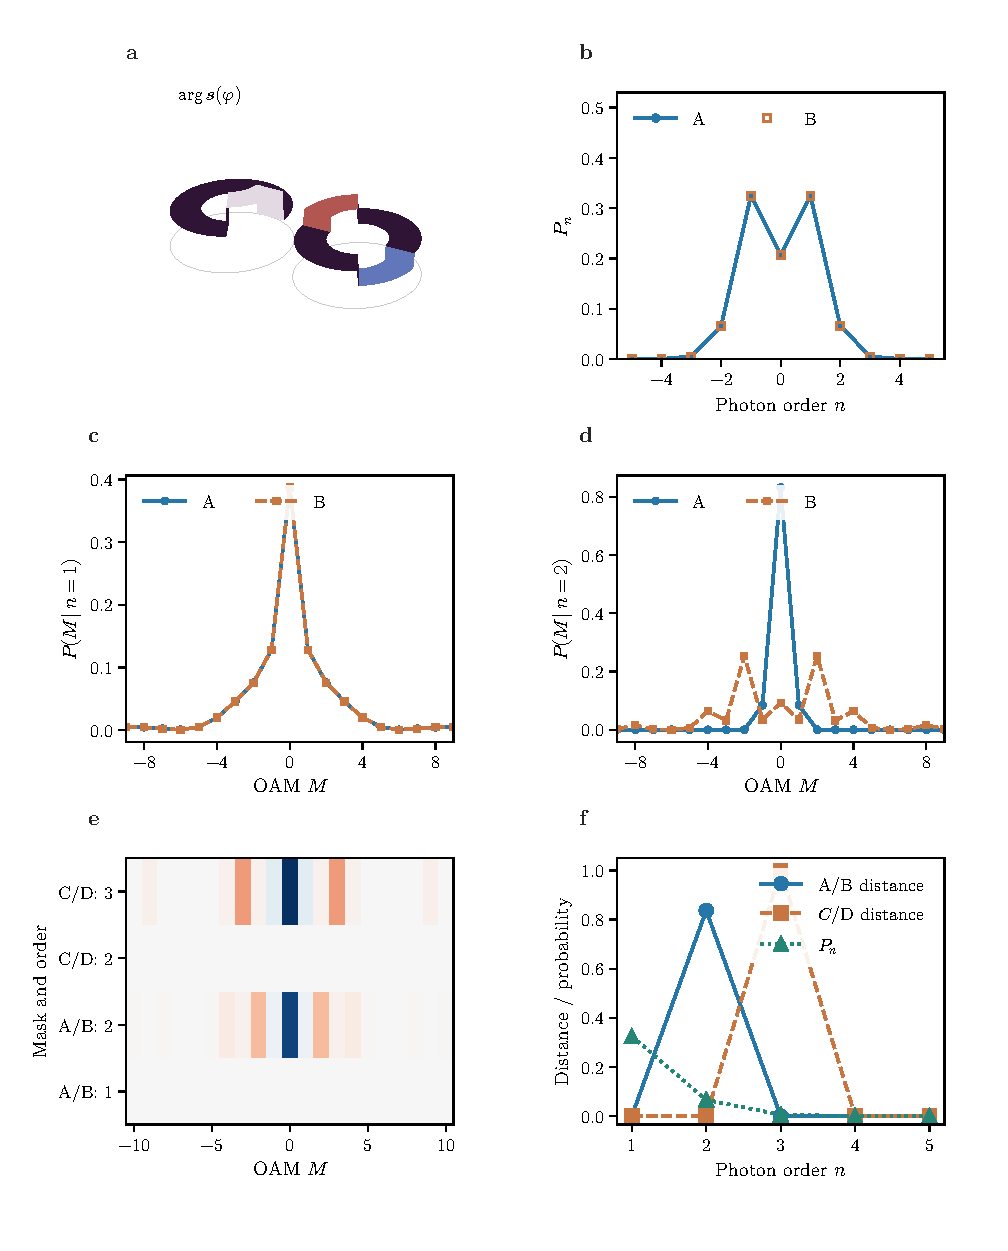
\includegraphics[width=0.96\linewidth,height=0.70\textheight,keepaspectratio]{oam_angular_homometry.pdf}
\caption{\textbf{多光子能量--OAM 读出解除角同距简并。} (a) 将六扇区相位纹理 A、B 的相位值编码为高度和循环色，三维高度只是 $\arg s/\pi$ 的几何显示，并非真实纳米结构起伏；(b) 两组角场的完整能量边带概率严格重合；(c) 一光子条件 OAM 概率也重合；(d) 双光子条件 OAM 谱显著分开；(e) 用同一 OAM 响应核比较 A/B 在一、二阶和 C/D 在二、三阶的逐模差异；(f) 两类角同距对的总变差距离随光子阶的变化，并与各阶事件概率比较。这里三维图、线谱和热图均由同一套六扇区精确系数计算。}
\label{fig:oam-angular-homometry}
\end{figure}

具体到各面板，(a) 两组原始角掩模均按\cref{eq:oam-six-sector-masks} 的六个等宽扇区取值；三维环面仅用 $z=0.62\arg(s_j)/\pi$ 表示扇区相位，高度不进入任何电子动力学。环的绘制半径为 $0.53\le r\le1.05$，相位由归一化循环色图显示，观察角为仰角 $27^\circ$、方位角 $-61^\circ$；这两个几何参数不影响谱值。(b) 取 $a=0.8$、$-5\le n\le5$，对 A/B 同时画 $P_n=J_n^2(1.6)$。(c,d) 对每个整数 $M\in[-250,250]$ 使用\cref{eq:oam-sector-exact-coeff} 的扇区解析积分，分别求 $n=1,2$ 条件谱；探测 OAM 核设为
\[
 K_{MM'}=\frac{\exp[-(M-M')^2/(2\sigma_M^2)]}
 {\sum_{R=-250}^{250}\exp[-(R-M')^2/(2\sigma_M^2)]},\qquad
 \sigma_M=\frac{1.1}{2\sqrt{2\ln2}},\qquad
 Q_n(M)=\sum_{M'}K_{MM'}|\widetilde{s^n}_{M'}|^2.
\]
$\sigma_M$ 用 OAM 量子数为单位，故对应 $1.1\hbar$ 的半高全宽。模截断造成的原始条件概率尾部流失在所画 $n\le5$ 范围内需由脚本检查；面板将模糊后的有限窗分布再次归一化后只显示 $|M|\le9$。(e) 同样用 $|M|\le250$ 计算四组差 $Q_B-Q_A$（$n=1,2$）和 $Q_D-Q_C$（$n=2,3$），纵轴四行只显示 $|M|\le10$；发散色标固定为 $[-0.8,0.8]$。(f) 以\cref{eq:oam-order-contrast} 求两对场在 $1\le n\le5$ 的总变差距离，同时显示 $P_n=J_n^2(1.6)$ 作为每阶事件的概率权重；纵轴将这两类无量纲量并置，不能据此把总变差距离解释成信噪比。脚本对 $|M|\le250$ 的有限窗重新归一化，因此图上报告的 $D_2$ 会随截断和 OAM 响应设置发生可计算的微小变化；它不是与仪器无关的实验常数。


实验的 OAM 排序器有有限分辨率，因而不能把理论中的 $P(M\mid n)$ 直接当成探测器计数。若以列归一的响应矩阵 $K_{MM'}$ 表示 OAM 模糊，则测得的条件概率是 $Q_n(M)=\sum_{M'}K_{MM'}P(M'\mid n)$。两种假设在第 $n$ 阶的可区分性可以定义为总变差距离
\begin{equation}
 D_n=\frac12\sum_M|Q_n^{(A)}(M)-Q_n^{(B)}(M)|.
 \label{eq:oam-order-contrast}
\end{equation}
$D_n$ 测量已经通过仪器响应之后的分布差别，但它不是事件信噪比。第 $n$ 阶的预期探测计数还乘以 $J_n^2(2a)$、总剂量和探测效率。因此提高光子交换阶数可以打开新的角相关信息，却同时遇到更稀少的计数；它给实验设计的是一个信息量与剂量的折衷，而不是越高阶越好。


还有一个看似矛盾的问题：即便某个高阶边带具有极大的 OAM 谱差异，它也可能因为几乎没有电子到达而不适合测量。为了定量讨论这种取舍，必须将“观测到该边带以后能否区分两种场”和“入射一个电子以后实际能获得多少证据”分开。前者由条件分布决定，后者必须重新乘上该边带的事件概率。

令 $H=A,B$ 表示两种候选角场，把仪器 OAM 响应作用于各自的条件分布后记为 $Q_n^H(M)$。这些分布在全部读出模上归一化为一。对一对分布定义经典重叠
\begin{equation}
 \mathcal B_n=\sum_M\sqrt{Q_n^A(M)Q_n^B(M)},
 \qquad 0\leq\mathcal B_n\leq1.
 \label{eq:oam-bhattacharyya-overlap}
\end{equation}
当 $\mathcal B_n=1$ 时，两个条件读出完全相同；减小到零则代表在理想单次条件读出中具有不重合的支持集。与总变差距离 $D_n$ 不同，$\mathcal B_n$ 直接进入有限剂量的判别概率上界。另一方面，不能把 $\mathcal B_n$ 当作材料性质：它依赖探测器响应、OAM 收集窗口，以及是否将其余端点都合并成一个读出事件。

仪器模糊为何使区分变得困难，也可以不依赖数值图而严格证明。对任何非负、列归一的响应 $K_{Mm}$，柯西--施瓦茨不等式逐个读出端点给出
\begin{align*}
 &\sqrt{\Big(\sum_mK_{Mm}p_m\Big)\Big(\sum_mK_{Mm}q_m\Big)}
 \;\geq\;\sum_m K_{Mm}\sqrt{p_m q_m},\\
 &\sum_M\sqrt{(Kp)_M(Kq)_M}\;\geq\;
 \sum_m\sqrt{p_mq_m}\sum_MK_{Mm}
 =\sum_m\sqrt{p_mq_m}.
\end{align*}
因此 $\mathcal B_n$ 在随机模糊下不能减小；同时总变差距离也不会增加。分辨率越差，理论上的角纹理差别越难转化成已经采集到的电子计数差别。

设实验同时收集第 $\pm n$ 两条对称能量边带，角掩模仍满足 $|s|=1$，OAM 响应关于 $M\mapsto-M$ 对称。由于 $s^{-n}=\overline{s^n}$，两条能量符号的条件谱互为 OAM 镜像，具有相同的 $\mathcal B_n$。在此模型中，单个指定正能量边带的总概率是 $w_n=J_n^2(2a)$。若只保留正整数阶数集合 $\mathcal S$ 中的两个能量符号和对应 OAM，其余所有结果只合并为一个“未选中”记录，则这个合并事件在两种候选场下都具有概率
\[
 p_H(\varnothing)=1-2\sum_{n\in\mathcal S}w_n,
 \qquad p_H(\pm n,M)=w_nQ_{\pm n}^H(M).
\]
注意 $p_H(\varnothing)$ 在两种假设下相同，并不意味着它在样本统计中不存在；大量电子未进入所选边带，恰恰会降低每个入射电子包含的判别信息。把全部互斥事件的平方根概率逐项相乘并求和，得到\emph{每个入射电子}的分布重叠
\begin{equation}
 \Lambda_{\mathcal S}=
 1-2\sum_{n\in\mathcal S}J_n^2(2a)(1-\mathcal B_n),
 \qquad
 \Gamma_{\mathcal S}=-\ln\Lambda_{\mathcal S}.
 \label{eq:oam-information-exponent}
\end{equation}
$\Gamma_{\mathcal S}$ 是由经典 Bhattacharyya 重叠定义的可计算判别指数，并非一般最优 Chernoff 指数。它同时记住两件事：即便 $1-\mathcal B_n$ 很大，当 $J_n^2(2a)$ 很小时，该阶对实验判别的贡献仍可忽略。

对于 $N_{\mathrm e}$ 个独立入射电子且两种假设先验各占一半，最优二元判决的平均错误概率为
\[
 P_{\mathrm{err}}(N_{\mathrm e})=
 \frac12\sum_{\vb y}\min\{p_A(\vb y),p_B(\vb y)\},
\]
其中 $\vb y$ 是整串实验记录。逐项使用 $\min\{u,v\}\leq\sqrt{uv}$，再利用各次实验独立性，就可把 $N_{\mathrm e}$ 维的概率求和分解为单次记录重叠的乘积，得到
\begin{equation}
 P_{\mathrm{err}}(N_{\mathrm e})
 \leq\frac12\Lambda_{\mathcal S}^{N_{\mathrm e}}
 =\frac12\ee^{-N_{\mathrm e}\Gamma_{\mathcal S}}.
 \label{eq:oam-error-bound}
\end{equation}
所以要让\emph{这条上界}低于指定容许值 $\epsilon$，一个充分的入射电子数是
\begin{equation}
 N_{\mathrm e}^{\mathrm{ub}}(\epsilon)
 =\left\lceil\frac{\ln(1/2\epsilon)}{\Gamma_{\mathcal S}}\right\rceil.
 \label{eq:oam-dose-sufficient}
\end{equation}
这是保证判别错误上界的\emph{充分剂量}，不是实际贝叶斯最优测量所必需的最小剂量。若电子计数相关、探测效率随相位变化或不同扇区的径向束流权重并不均匀，上面的单电子分布必须重新建模，不能继续直接套用这个式子。

六扇区 A/B 掩模显示了这种取舍的非单调性。它们的条件 OAM 读出只在 $n\equiv2\pmod4$ 的光子交换阶首次获得区分能力；第一、第三、第四与第五阶即使测到许多电子也不提供这对掩模的判别信息。取 $a=0.8$、OAM 模糊半高全宽 $1.1\hbar$ 时，第二阶的总变差距离约为 $0.837$，而第六阶虽然有相同条件对比，事件概率却只有约 $1.1\times10^{-7}$。当 $a$ 接近 $J_2(2a)$ 的首个非零零点时，第二阶的入射剂量效率骤降，此时第六阶可能接管测量；进一步在 $a=3$ 时，联合使用两组正负能量阶的判别上界可以比单选其中一组下降得更快。因而“应测量哪一阶”不是一句“尽可能高阶”可以回答的问题，它取决于具体耦合、探测分辨率和剂量。

\begin{figure}[!htbp]
\centering
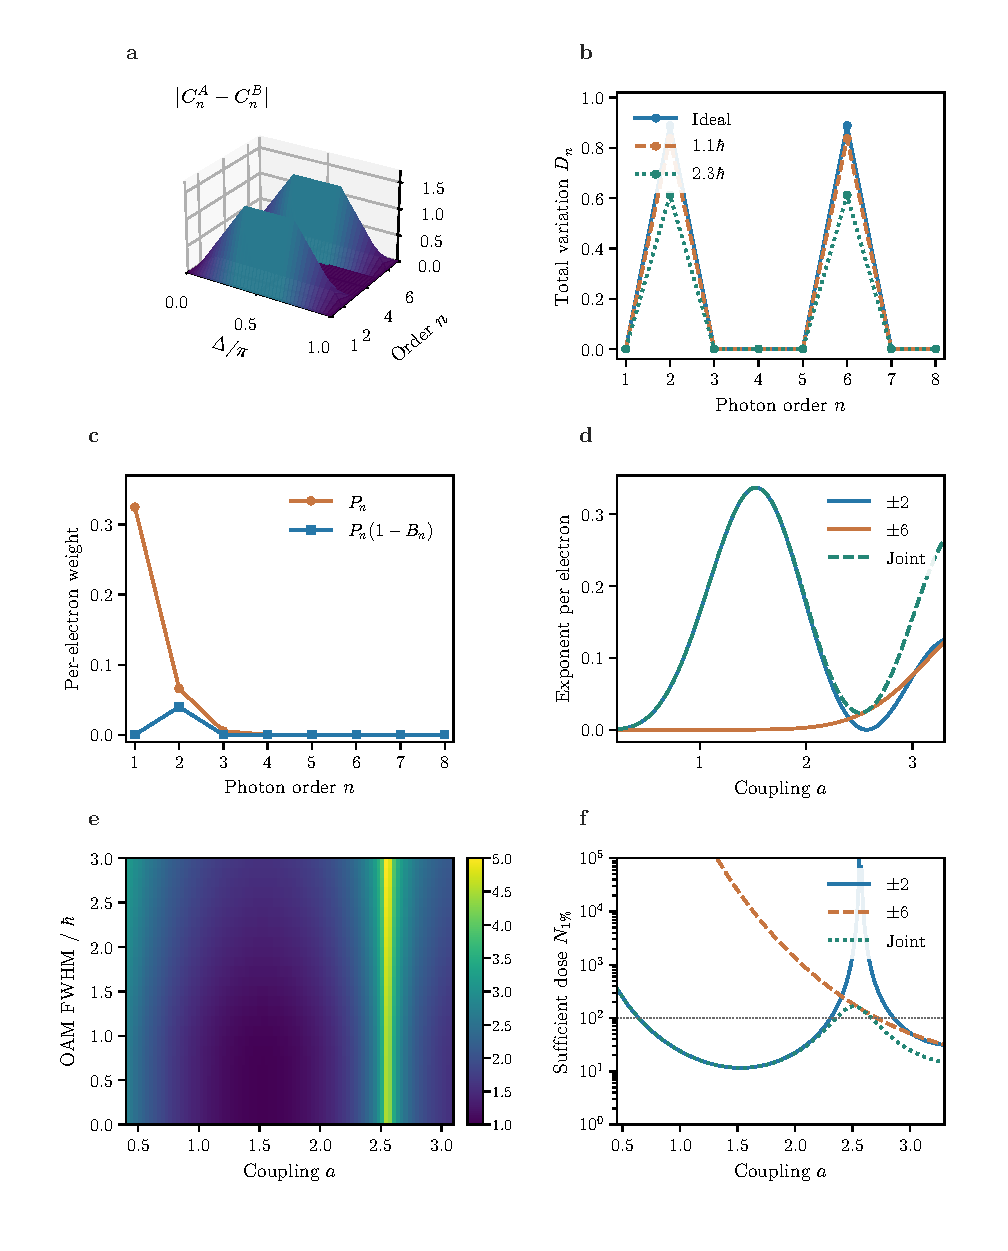
\includegraphics[width=0.96\linewidth,height=0.70\textheight,keepaspectratio]{oam_information_budget.pdf}
\caption{\textbf{从角同距的可区分性到实际电子剂量。} (a) 三维曲面绘制六扇区 A/B 两场角相位增量相关函数的模差 $|C_n^A(\Delta)-C_n^B(\Delta)|$，三轴都是模型给出的数学观测量，并非装饰性合成晶格；(b) 不同 OAM 分辨率下的各阶条件总变差距离，只有选择规则允许的阶数出现峰值；(c) 比较 $a=0.8$ 时边带事件概率 $P_n$ 与有效单边带权重 $P_n(1-\mathcal B_n)$；(d) 将第 $\pm2$ 阶、第 $\pm6$ 阶及其联合读出的每电子判别指数作为耦合强度的函数，贝塞尔零点附近可见测量阶数切换；(e) 同时扫描耦合与 OAM 模糊，绘制仅收集 $\pm2$ 阶时使等先验错误概率\emph{上界}低于 $1\%$ 的充分入射剂量 $\log_{10}N_{\mathrm e}^{\mathrm{ub}}$，色标截断处不意味着剂量趋于有限常数；(f) 对同样三种边带选择扫描耦合强度，展示使理论错误概率上界低于 $1\%$ 所需的入射电子剂量；在贝塞尔零点附近所需剂量显著增加。全部曲面、线谱和热图均由同一六扇区 Fourier 精确系数及指定随机探测响应计算。}
\label{fig:oam-information-budget}
\end{figure}

本图的两个候选场完全沿用\cref{eq:oam-six-sector-masks} 的 A/B 六扇区相位因子，均取恒定径向振幅、均匀角向入射波、初始 OAM $M=0$。对所有面板，条件 OAM 理想概率先由\cref{eq:oam-sector-exact-coeff} 解析求得，在 $-250\le M\le250$ 上积分截断，探测矩阵采用前图定义的离散高斯列归一模型；对每个条件谱在该有限窗口内再次归一化。没有加入场的无序、材料吸收、能量探测噪声或未知分类背景。(a) 以 $n=1,\ldots,7$ 和 $\Delta\in[0,\pi]$ 的 $121$ 个均匀点，直接计算
\[
 C_n^H(\Delta)=\sum_{M=-250}^{250}
 |\widetilde{(s_H)^n}_M|^2\ee^{\ii M\Delta},\qquad
 Z_n(\Delta)=|C_n^A(\Delta)-C_n^B(\Delta)|.
\]
绘制 $Z_n$ 的三维曲面；三维纵轴表示计算得到的相位增量相关差异，不是电子的第三个末态量子数。视角取仰角 $26^\circ$、方位角 $-58^\circ$，显示高度范围 $[0,1.7]$。(b) 在 $n=1,\ldots,8$ 分别使用理想无模糊响应及 FWHM 为 $1.1\hbar,2.3\hbar$ 的 OAM 高斯分辨率，计算\cref{eq:oam-order-contrast} 中的 $D_n$。(c) 固定 $a=0.8$、FWHM $=1.1\hbar$，对 $n=1,\ldots,8$ 绘制 $J_n^2(1.6)$ 和 $J_n^2(1.6)(1-\mathcal B_n)$；这里只记录单个正能量边带的权重，没有把负能量边带计数重复乘入。(d) 固定同一分辨率，以 $a\in[0.22,3.3]$ 的 $116$ 个均匀点，用\cref{eq:oam-information-exponent} 分别取 $\mathcal S=\{2\},\{6\},\{2,6\}$，三者都收集对应的正负能量边带。(e) 取 $a\in[0.40,3.10]$ 的 $85$ 点和 OAM 分辨率 FWHM $\in[0,3]\hbar$ 的 $27$ 点，以 $\mathcal S=\{2\}$ 和 $\epsilon=0.01$ 计算\cref{eq:oam-dose-sufficient} 的充分入射剂量。热图显示 $\log_{10}$ 剂量，颜色截断在 $[1,5]$；离散插图用未取整的连续剂量表达式，实际剂量取其向上整数。(f) 固定 OAM 分辨率 FWHM $=1.1\hbar$，取 $a\in[0.45,3.3]$ 的 301 点，根据\cref{eq:oam-dose-sufficient} 对比三组 $\mathcal S$ 的 $1\%$ 错误概率充分剂量。纵轴为对数尺度，只绘制 $1\leq N_{1\%}\leq10^5$ 的有效区域；水平参考线表示 100 个入射电子。所有图中的两假设具有相同的完整能量谱，因此未收集事件在两种假设下概率相同；若未来将 $|\beta(\varphi)|$ 的幅度起伏纳入模型，必须同时更新未收集事件的概率与相应判别公式。


上述讨论只涉及角相位在不同能量阶中的读出。除此之外，端点量子数还可能抹去完全不同的散射历史。

\section{多路径干涉}
另一个与角同距性互补的困难发生在多色、多角动量通道的\emph{复合交换历史}中。同一电子末态可能由不同的事件组合到达，而电子能量和 OAM 只保留这些事件的总和。把每种独立可调相的基本事件记为一个整数计数 $h_j$，列成 $\vb h\in\mathbb Z^k$，再把事件末态荷排成整数矩阵 $A$。完整可观测端点为 $\vb x=A\vb h$；若两条历史 $\vb h,\vb h'$ 到达同一端点，则
\begin{equation}
 A(\vb h-\vb h')=0,
 \qquad L=\ker_{\mathbb Z}A.
 \label{eq:oam-relation-lattice}
\end{equation}
关系晶格 $L$ 所记录的不是额外的空间维度，而是\emph{被端点量子数抹去的历史差别}。若事件 $j$ 具有可调相位 $\theta_j$，到达固定端点 $\vb x$ 的各历史相干和为
\begin{equation}
 \mathcal A_{\vb x}(\boldsymbol\theta)
 =\sum_{\vb h:A\vb h=\vb x}
 a_{\vb h}\,\ee^{\ii\vb h\cdot\boldsymbol\theta},
 \qquad P_{\vb x}=|\mathcal A_{\vb x}|^2,
 \label{eq:oam-history-amplitude}
\end{equation}
其中 $a_{\vb h}$ 还包括传播子、时间排序、矩阵元和中间态相位。在平方展开时，每对历史的交叉项携带 $\ee^{\ii(\vb h-\vb h')\cdot\boldsymbol\theta}$。故\emph{只有} $\vb h-\vb h'\in L$ 的相位谐波可能出现在固定端点的计数中；属于 $L$ 仅保证运动学上允许，具体振幅还可以因路径不存在、动力学相消或环境失相干而为零。

用三个实验上可分辨驱动事件给出最小的二维例子：
\begin{equation}
 \vb g_1=(1,+1),\quad \vb g_2=(1,-1),\quad \vb g_3=(2,0),\qquad
 A=\begin{pmatrix}1&1&2\\1&-1&0\end{pmatrix}.
 \label{eq:oam-three-channel-matrix}
\end{equation}
直接计算 $A(1,1,-1)^{\mathsf T}=0$，故一条 $\vb g_1$ 与一条 $\vb g_2$ 的复合路径和一次 $\vb g_3$ 直接跃迁到达同一端点 $(2,0)$。循环相位的独立组合是
\begin{equation}
 \Phi=\theta_1+\theta_2-\theta_3.
 \label{eq:oam-primitive-loop-phase}
\end{equation}
与两条线性独立跳跃所形成的无限 Bravais 晶格不同，第三条跳跃构成了实际闭合回路，$\Phi$ 不能由四个端点的任意局域相位重定义同时消去。因此扫描它能够调制端点人口。

为了从一般关系判据落到真正可复算的动力学，取有限四态基 $\{|0\rangle,|+\rangle,|-\rangle,|f\rangle\}$，分别表示 $(0,0),(1,+1),(1,-1),(2,0)$。非零的向前跃迁矩阵元取
\begin{equation}
 H_{+,0}=g_1\ee^{\ii\theta_1},\quad
 H_{-,0}=g_2\ee^{\ii\theta_2},\quad
 H_{f,+}=g_2\ee^{\ii\theta_2},\quad
 H_{f,-}=g_1\ee^{\ii\theta_1},\quad
 H_{f,0}=g_3\ee^{\ii\theta_3},
 \label{eq:oam-endpoint-four-state}
\end{equation}
其余反向矩阵元取厄米共轭。令 $\tau$ 为无量纲作用时间，用完整的 $\ee^{-\ii H\tau}$ 演化而不是只靠最低阶微扰。为了理解回路相位为何出现，可以把末态振幅展开到二阶：
\begin{align*}
 \langle f|\ee^{-\ii H\tau}|0\rangle
 &= -\ii\tau H_{f0}-\frac{\tau^2}{2}
 \sum_j H_{fj}H_{j0}+O(\tau^3)\\
 &= -\ii\tau g_3\ee^{\ii\theta_3}
 -\tau^2g_1g_2\ee^{\ii(\theta_1+\theta_2)}+O(\tau^3).
\end{align*}
二阶项中的系数没有额外的 $1/2$，因为 $|+\rangle$ 和 $|-\rangle$ 两条时间有序路径各贡献一次。保留领先的交叉项，得到
\begin{equation}
 P_f(\Phi)=\tau^2g_3^2+2\tau^3g_1g_2g_3\sin\Phi+O(\tau^4).
 \label{eq:oam-loop-weak-response}
\end{equation}
$\sin\Phi$ 而非 $\cos\Phi$ 的相位偏移，来自直接一跳和复合两跳各自的 Dyson 因子 $-\ii$ 与 $(-\ii)^2$。完整数值计算保留全部高阶重访路径，不能在强耦合区继续用这个低阶表达式代替。

如果增加一个\emph{真正可分辨}的末态标签，使直接路径到达 $|f,\mathrm d\rangle$、复合路径到达与之正交的 $|f,\mathrm c\rangle$，而探测器只统计二者的总人口，则
\begin{equation}
 P_f=P_{f,\mathrm d}+P_{f,\mathrm c},\qquad
 \langle f,\mathrm d|f,\mathrm c\rangle=0.
 \label{eq:oam-graded-endpoint}
\end{equation}
此时交叉项严格消失。关系晶格的语言将其写成：增加新端点荷 $B$ 以后，只有 $L\cap\ker B$ 内的历史差仍可干涉。必须强调，“给路径一个不同名称”并不会产生正交标签；只有物理上可区分的环境记录、光子态或新增荷真正保留了哪条路径的信息，才有这种严格的结构性关断。它和仅把某个驱动幅度调到零是不同的实验机制。

\begin{figure}[!htbp]
\centering
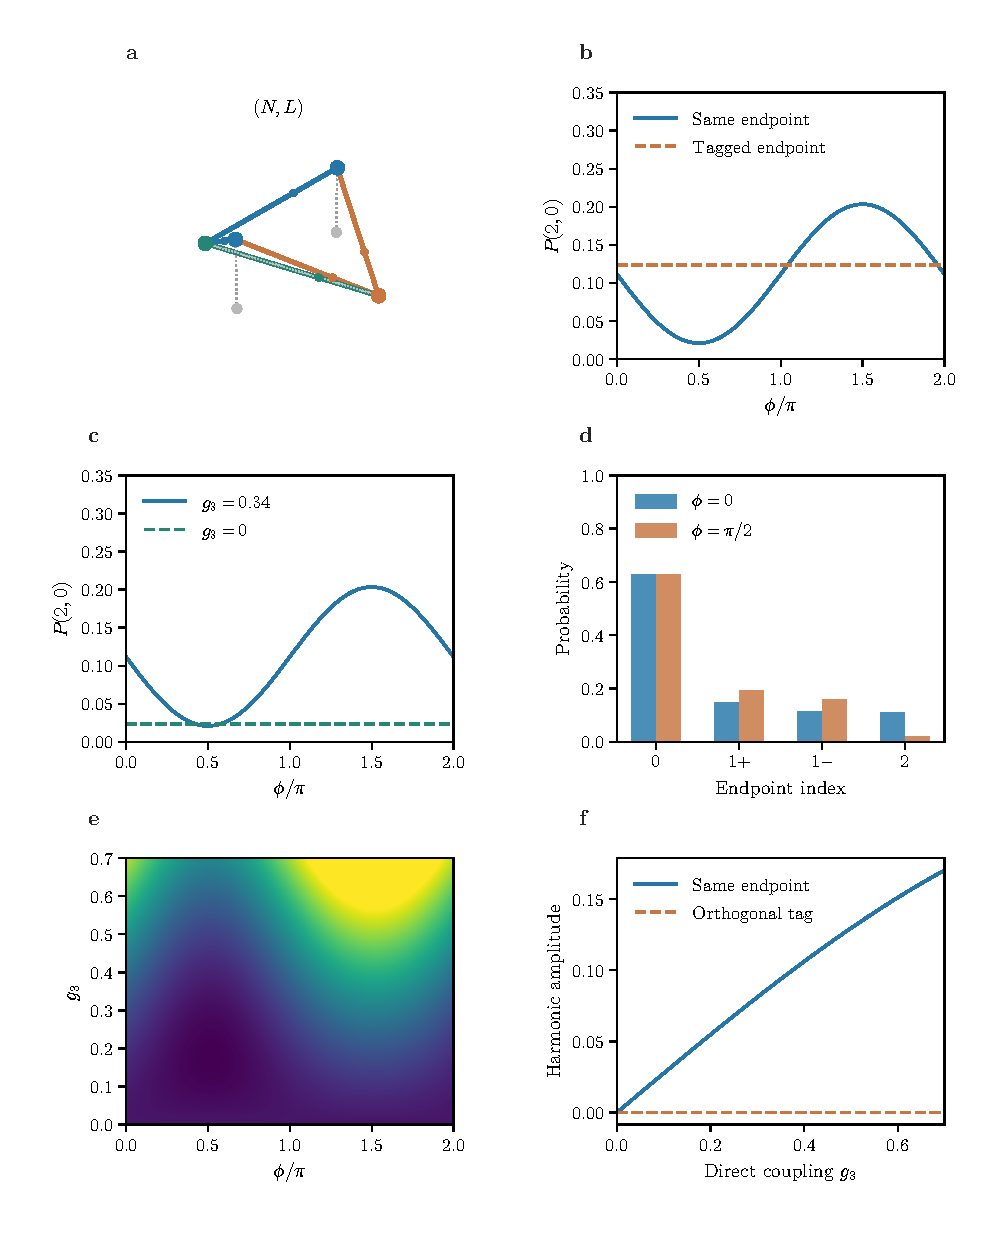
\includegraphics[width=0.96\linewidth,height=0.70\textheight,keepaspectratio]{oam_endpoint_histories.pdf}
\caption{\textbf{端点关系晶格与多路径相干开关。} (a) 在真实 $(N,L)$ 整数坐标上表示三种基本跃迁；三维图中的辅助高度只用来分开中间路径，并非第三个电子量子数。(b) 直接路径和双步路径到达同一端点时，完整有限维幺正演化的末态人口随回路相位变化；增加正交末态标签后相位调制消失。(c) 关闭直接通道 $g_3$，同一原始模型的相位响应变平坦；(d) 比较两个相位下全部四个端点的概率；(e) 扫描直接通道强度与回路相位的二维响应；(f) 从严格相位 Fourier 变换提取一阶谐波，与带正交标签的结构零对照。所有概率都由同一个厄米矩阵的矩阵指数求得，不是手工设置干涉条纹。}
\label{fig:oam-endpoint-histories}
\end{figure}

数值实现中，四态基按 $|0\rangle,|+\rangle,|-\rangle,|f\rangle$ 排列，采用\cref{eq:oam-endpoint-four-state} 的所有正向矩阵元及其厄米共轭，取 $g_1=0.43$、$g_2=0.38$、$g_3=0.34$、$\tau=1$，除单独扫描的 $\theta_3$ 外设 $\theta_1=\theta_2=0$。(a) 节点真实坐标为 $(N,L)=(0,0),(1,+1),(1,-1),(2,0)$；第三个绘图坐标只是将中间节点从平面抬升 $0.8$ 以显露全部跃迁，视角为仰角 $27^\circ$、方位角 $-58^\circ$。(b) 用 $\ee^{-\ii H\tau}$ 严格计算初态 $|0\rangle$ 到 $|f\rangle$ 的概率，在 $\theta_3\in[0,2\pi]$ 取 $121$ 点；作为比较的带标签模型扩成五态，使一次直接跃迁到达 $|f,\mathrm d\rangle$、复合跃迁到达 $|f,\mathrm c\rangle$，报告这两个正交末态的概率之和。(c) 原四态哈密顿量不变而令 $g_3=0$，展示缺少第三跳跃以后回路相位不再可观测。(d) 在 $\theta_3=0,\pi/2$ 分别计算四个端点概率，概率之和必须等于一。(e) 固定 $g_1,g_2,\tau$，在 $g_3\in[0,0.7]$ 的 $42$ 点和 $\theta_3\in[0,2\pi)$ 的 $64$ 点取样，并以 $[0,0.4]$ 的共同色标显示 $P_f$。(f) 对 $g_3\in[0,0.7]$ 的 $31$ 点扫描，以等间隔 $64$ 个相位求 Fourier 系数 $c_1=64^{-1}\sum_{j=0}^{63}P_f(2\pi j/64)\ee^{-2\pi\ii j/64}$，绘制 $2|c_1|$；同一运算施于带正交末态标签的模型，应在浮点精度内给出零。所有面板都使用厄米哈密顿量，没有假设非厄米增益，也未把辅助绘图高度当作第三个实验端点荷。


这两种新读出解决的是不同层次的不可辨识性：高阶能量--OAM 谱读出角相位差的高阶矩，端点关系谱学读出多条交换历史的相位差。它们都超出只测量 $\sum_M P_{nM}$ 的传统能量 PINEM，却不要求修改量子力学的基本原则。前者需要控制初态 OAM、测量窗口与高阶边带剂量；后者还需逐通道标定驱动相位并证明各路历史确实相干。将二者用于真实材料时，必须先从 Maxwell 场与轨迹积分算出角耦合，再加入 OAM 响应和环境记录；这里只把这些新的信息通道作为严格定义的有效模型预言。


上一段的关系晶格仍留下一个实验上十分尖锐的问题：如果三束光并不是绝对相位稳定的，闭合回路的干涉是否一定会消失？初学时容易把答案想成“每束激光都要稳定”，但哈密顿量真正依赖的是\cref{eq:oam-primitive-loop-phase} 的\emph{关系相位}。因此我们不妨先从这一简单、能够测量的量出发，逐步分析更复杂的相位噪声。

把三条驱动的随机相位写为 $\vb\theta=\vb\theta_0+\delta\vb\theta$，其关系向量是 $\vb u=(1,1,-1)^{\mathsf T}$。对同一完整能量--OAM 末态 $(2,0)$，无论是微扰区还是强耦合区，只要哈密顿量保持\cref{eq:oam-endpoint-four-state} 的连接结构，它的概率就是一个 $2\pi$ 周期函数
\begin{equation}
 P_f(\Phi)=\sum_{h\in\mathbb Z}c_h\ee^{\ii h\Phi},\qquad
 c_h=\frac1{2\pi}\int_0^{2\pi}P_f(\Phi)\ee^{-\ii h\Phi}\,\dd\Phi,
 \qquad \Phi=\vb u^{\mathsf T}\vb\theta.
 \label{eq:oam-noise-relation-fourier}
\end{equation}
关系谐波 $h$ 对应净交换历史之差 $h\vb u$。这句话的实验含义是：对 $\Phi$ 作相位循环扫描，再 Fourier 分析末态计数，可以直接读出哪些关系谐波仍具有相干性；但仅有端点谱并不能恢复所有内部历史的复振幅。

现在假设不同电子到达时采样到的相位误差服从均值为零、协方差为 $\Sigma$ 的多元高斯分布。由于 $\delta\Phi=\vb u^{\mathsf T}\delta\vb\theta$，其方差不是三个单独方差的简单总和，而是
\begin{equation}
 V_{\Phi}=\operatorname{Var}(\delta\Phi)=\vb u^{\mathsf T}\Sigma\vb u.
 \label{eq:oam-noise-projected-covariance}
\end{equation}
沿每个电子的随机相位轨迹先算概率再取平均，利用高斯特征函数 $\langle\ee^{\ii h\delta\Phi}\rangle=\ee^{-h^2V_\Phi/2}$，得到一个对\emph{完整有限时间幺正演化}成立的等式：
\begin{equation}
 \overline P_f(\Phi)=\sum_{h\in\mathbb Z}c_h\,
 \exp\!\left(\ii h\Phi-\frac{h^2}{2}\vb u^{\mathsf T}\Sigma\vb u\right).
 \label{eq:oam-noise-filter-exact}
\end{equation}
它并未把 $P_f$ 近似为正弦曲线；所有高阶重访和多次散射路径已包含在系数 $c_h$ 中。这也区分了两个容易混淆的过程：增加一个可解析的\emph{正交末态荷}会在结构上禁止某些历史的交叉项；相位随机化则使允许的谐波连续衰减。若 $\Sigma\vb u=0$，即使 $\Sigma$ 的其他特征值很大，关系相位仍无噪声。这是由协方差半正定性和零空间直接推出的结论，而非额外的拓扑保护。

一个具体的锁相模型能把上述数学事实变成可以调节的实验参数。令 $x,y,z$ 相互独立且分别服从 $\mathcal N(0,\sigma^2)$、$\mathcal N(0,\sigma^2)$ 和 $\mathcal N(0,1)$，并设置
\begin{equation}
 \delta\theta_1=x,\qquad\delta\theta_2=y,\qquad
 \delta\theta_3=\lambda(x+y)+\epsilon z,\qquad
 V_\Phi=2(1-\lambda)^2\sigma^2+\epsilon^2.
 \label{eq:oam-noise-correlated-locking}
\end{equation}
$\lambda=1$ 表示第三路的光学相位随前两路之和漂移，$\epsilon$ 则是不可共同抵消的残余误差。此时只有 $\epsilon^2$ 决定关系谐波的衰减，尽管第三路的\emph{绝对相位}本身可能比任何一路都更不稳定。相反，三路独立且每路标准差同为 $\sigma$ 时，$V_\Phi=3\sigma^2$。这种保护依赖物理相位锁定与实际的末态交换关系，不意味着任何三束不相关激光都自动满足它。

\begin{figure}[!htbp]
\centering
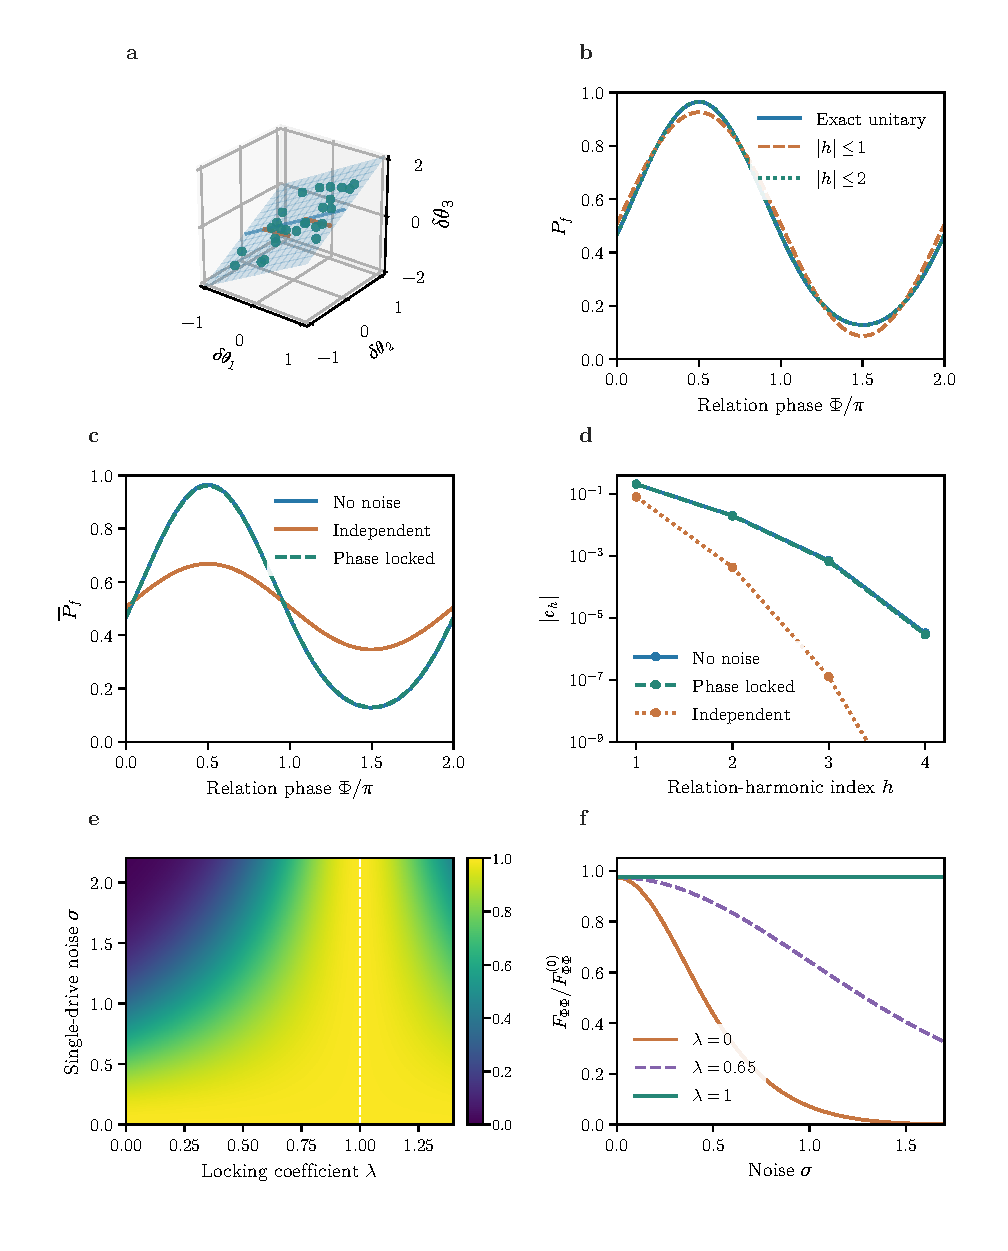
\includegraphics[width=0.96\linewidth,height=0.70\textheight,keepaspectratio]{relation_noise_geometry.pdf}
\caption{\textbf{关系晶格的相位噪声零空间与可读出干涉。} (a) 在三个\emph{驱动相位误差}构成的参数空间中绘出 $\delta\theta_3=\delta\theta_1+\delta\theta_2$ 的保护平面；点为锁相噪声抽样，面外的箭头沿关系向量 $\vb u$。这不是三维空间中的电子轨道。(b) 四态厄米哈密顿量的精确末态人口及截断到一阶、二阶关系谐波的 Fourier 重构。(c) 同等单路噪声下，三路独立与关系相位锁定的系综平均人口。(d) 不同谐波阶数的绝对 Fourier 系数，显示 $h^2$ 噪声滤波。(e) 扫描锁相系数 $\lambda$ 和单路相位噪声 $\sigma$，颜色为一阶谐波保留率。(f) 在固定工作相位处，用完整 Bernoulli 计数模型计算每入射电子的关系相位 Fisher 信息，与无噪声的数值比较。三维坐标是相位参数，不是另设的物理维度。}
\label{fig:oam-relation-noise-geometry}
\end{figure}

为了复现\cref{fig:oam-relation-noise-geometry}，使用\cref{eq:oam-endpoint-four-state} 中的 $g_1=0.43$、$g_2=0.38$、$g_3=0.34$，但选较长的无量纲作用时间 $\tau=2.5$，使一阶以外的关系谐波在图上可见。取 $512$ 个等间距 $\Phi\in[0,2\pi)$ 点，用 $4\times4$ 厄米矩阵的 $\ee^{-\ii H\tau}$ 精确计算 $P_f$ 并作离散 Fourier 变换；这不是弱作用时间的 Dyson 截断。图 (a) 用 $\lambda=1$ 的锁相平面和固定随机种子 $101$ 的点作三维显示；(b) 由 $c_h$ 分别只保留 $|h|\le1$ 和 $|h|\le2$，与全解对照；(c,d) 对独立噪声取 $\sigma=0.8$，对锁相噪声取 $\lambda=1,\epsilon=0.12$，采用\cref{eq:oam-noise-filter-exact}；(e) 扫描 $\lambda\in[0,1.4]$ 的 $85$ 点和 $\sigma\in[0,2.2]$ 的 $91$ 点，显示 $\exp[-V_\Phi/2]$。最后，若探测器只记录电子是否到达 $(2,0)$，每个电子是参数为 $\overline P_f$ 的 Bernoulli 试验，故
\begin{equation}
 F_{\Phi\Phi}^{\mathrm{(bin)}}=\frac{(\partial_\Phi\overline P_f)^2}{\overline P_f(1-\overline P_f)}.
 \label{eq:oam-noise-binary-fisher}
\end{equation}
图 (f) 先在 $128$ 个工作相位中选择无噪声 Fisher 信息最大的一个，再保持该相位不动，以 $\sigma\in[0,1.7]$ 的 $70$ 点比较 $\lambda=0,0.65,1$，固定 $\epsilon=0.12$。这里的 Fisher 信息针对\emph{单一闭合回路相位}，并假定其他耦合已知；若同时估计三个绝对相位，只有关系方向可能从这一端点计数被辨认，不能把标量信息错误理解为可逆的三维 Fisher 矩阵。

上述零空间保护针对的是几路光学驱动的\emph{整体关系相位}。角同距测量还要求角向近场在不同位置保持相位相干。把六扇区复相位改为 $s_j\ee^{\ii\delta_j}$，其中 $\delta_j$ 的共同方差为 $\sigma^2$，不同扇区误差的等相关系数为 $0\le\rho\le1$；等相关模型的协方差为 $\Sigma^{\rm ang}_{jk}=\sigma^2[(1-\rho)\delta_{jk}+\rho]$。设第 $n$ 阶 Fourier 模振幅为 $a_{nM}$，先对每次电子散射的\emph{概率}取噪声平均，而不是先平均复振幅，展开模平方并分别处理 $j=k$ 和 $j\ne k$，得到
\begin{align}
 \overline{P}(M\mid n)&=\frac{\operatorname{sinc}^2(M\pi/6)}{36}
 \sum_{j,k=0}^{5}s_j^n(s_k^*)^n\ee^{-\ii M(\varphi_j-\varphi_k)}
 \exp\!\left[-\frac{n^2}{2}\operatorname{Var}(\delta_j-\delta_k)\right]\notag\\
 &=q_n|\widetilde{s^n}_M|^2+(1-q_n)\frac{\operatorname{sinc}^2(M\pi/6)}{6},\qquad
 q_n=\exp[-n^2\sigma^2(1-\rho)],\quad \varphi_j=(j+\tfrac12)\pi/3.
 \label{eq:oam-sector-dephasing-exact}
\end{align}
这条等式只使用了高斯相位误差的特征函数与六扇区精确 Fourier 系数，并不假设某个高阶能量边带概率可以当作总电子计数。若 $\rho=1$，所有扇区一起漂移，相对角相位不变，整个 OAM 谱严格不变；若 $\rho=0$，跨扇区相干的衰减因子变为 $\ee^{-n^2\sigma^2}$。因此高阶读出虽然能打破低阶同距简并，却同时放大局部角相位噪声的影响。两者放在一起，才构成真正有用的实验设计准则。

\begin{figure}[!htbp]
\centering
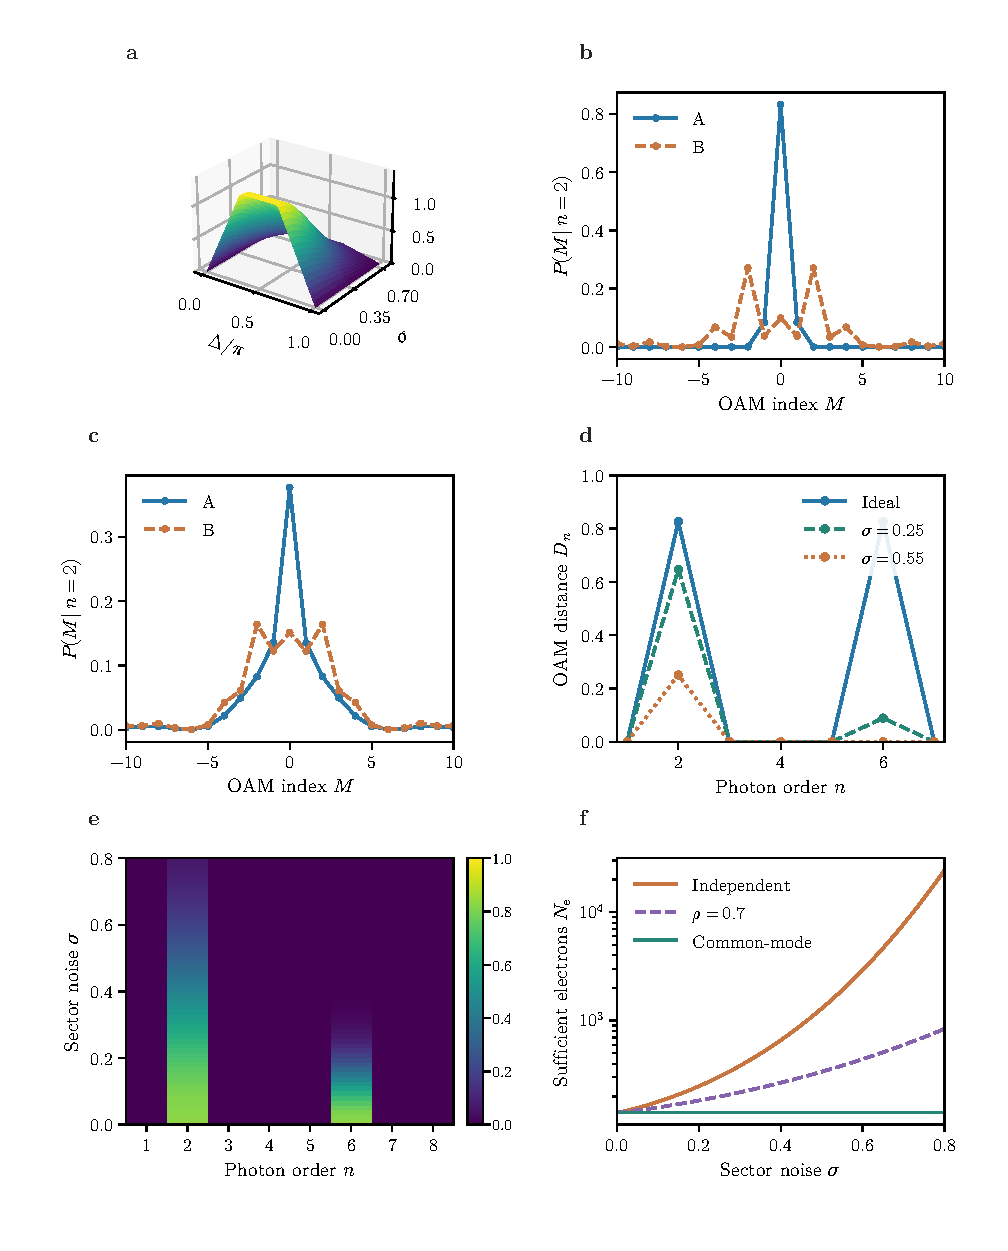
\includegraphics[width=0.96\linewidth,height=0.70\textheight,keepaspectratio]{oam_sector_noise.pdf}
\caption{\textbf{高阶角相位信息与噪声关联的互补取舍。} (a) 由精确角自相关求得的 $|C_2^A(\Delta)-C_2^B(\Delta)|$ 随角位移和独立扇区噪声的三维曲面；高度是数学相关函数对比，不是样品高度。(b,c) 理想情况与 $\sigma=0.55$ 时的正二阶条件 OAM 谱，都通过相同 OAM 模糊及收集窗口。(d) 按光子交换阶数显示条件总变差距离 $D_n$ 的衰减，揭示 $n^2$ 相位噪声代价。(e) $D_n$ 关于阶数与扇区噪声的热图，未出现的阶数并非未扫描。(f) 采用入射电子计数（而非后选择事件）定义的 $1\%$ 判别错误率\emph{上界}所需充分剂量，比较独立、部分关联和共同漂移。图中所有概率都由同一六扇区解析 Fourier 系数计算，不使用概念渲染。}
\label{fig:oam-sector-noise}
\end{figure}

\cref{fig:oam-sector-noise} 的数值条件保持与前面的高阶角同距算例一致：掩模取\cref{eq:oam-six-sector-masks}，OAM 理论求和保留 $-120\le M\le120$，探测器用列归一化高斯响应，模分辨率 FWHM 为 $1.1\hbar$，成功检出概率 $\eta_{\rm d}=0.72$，只接纳 $|M|\le12$。图 (a) 取 $50$ 个 $\Delta\in[0,\pi]$、$29$ 个 $\sigma\in[0,0.75]$，用\cref{eq:oam-sector-dephasing-exact} 的两假设谱差计算相关函数；(b,c) 分别取 $\sigma=0,0.55$；(d) 在 $n=1,\ldots,7$ 比较 $\sigma=0,0.25,0.55$；(e) 以 $56\times8$ 网格扫描 $\sigma\in[0,0.8],n=1,\ldots,8$。对图 (f) 固定样品 $a=0.8$ 和只收集\emph{正二阶}边带，令 $p_M^H=J_2^2(2a)\eta_{\rm d}\sum_{M'}K_{MM'}\overline P_H(M'\mid2)$，所有未收集电子合并为 $p_\varnothing^H=1-\sum_{|M|\le12}p_M^H$，其中 $H=A,B$。两假设的逐电子 Bhattacharyya 重叠及充分剂量是
\begin{equation}
 \mathcal B=\sqrt{p_\varnothing^A p_\varnothing^B}
 +\sum_{|M|\le12}\sqrt{p_M^A p_M^B},\qquad
 \Gamma=-\ln\mathcal B,\qquad
 N_{\rm e}^{\rm suff}=\left\lceil\frac{\ln50}{\Gamma}\right\rceil.
 \label{eq:oam-sector-noise-dose}
\end{equation}
图 (f) 扫描 $55$ 个 $\sigma\in[0,0.8]$，并比较 $\rho=0,0.7,1$。该剂量是保证等先验单次决策误差\emph{上界}低于 $1\%$ 的充分值，不是实际最优误码率的精确值。随机相位噪声假设为每个入射电子重新采样的平稳高斯过程；若角向近场在整个实验期间缓慢漂移甚至固定成另一幅图案，必须改为条件模型或带时间相关性的统计反演，不能直接使用上述退相干平均。

把这两种噪声对照起来，可以形成一个以信息读出为中心的新设计思路：\emph{沿关系向量的噪声投影}决定复合交换历史的干涉是否保留，而\emph{不同角扇区之间的相位差}决定高阶 OAM 信息是否保留。这并非已经实验验证的新拓扑效应，也不保证一种具体架构能同时稳定这两个子空间；它只是从两篇研究手稿出发，通过严格的随机模型得到的\emph{可证伪预测}。真实实验还必须检查频率倍频相锁能否实现所需的 $\theta_3\simeq\theta_1+\theta_2$、角向近场对光学漂移的响应是否确如这里假设，以及探测器的模式混合是否随时间稳定。


前面得到的两个噪声定律还可以倒过来使用。假设我们可以主动扫描各个光学通道的相位，并且每个相位点积累足够多的电子计数，能否从干涉条纹本身诊断噪声来自哪种组合？这并不等同于通常所说的“把所有激光相位噪声都测出来”：电子端点只感受交换历史之间的相位差，因而只能重建与那些历史关系相联系的噪声投影。下面从一个比单闭合回路多出一个可控相位的最小例子，严格回答这个可辨识性问题。

取四种基本交换事件，分别携带能量--OAM 端点荷
\begin{equation}
 \vb g_1=(1,1),\quad \vb g_2=(1,-1),\quad
 \vb g_3=(2,0),\quad \vb g_4=(0,2),\qquad
 A_4=\begin{pmatrix}1&1&2&0\\1&-1&0&2\end{pmatrix}.
 \label{eq:oam-two-loop-charges}
\end{equation}
这里的第二个分量均以 $\hbar$ 为单位，$\vb g_4$ 在有效模型中表示一种不改变电子能量、但改变 OAM 的已标定作用通道；其微观光场实现并不由这个整数记账式保证。直接求整数核得到两个独立关系
\begin{equation}
 \vb u=(1,1,-1,0)^{\mathsf T},\qquad
 \vb v=(1,-1,0,-1)^{\mathsf T},\qquad
 A_4\vb u=A_4\vb v=0.
 \label{eq:oam-two-loop-basis}
\end{equation}
从 $\vb h_0=(0,1,1,1)^{\mathsf T}$ 出发，四组非负整数历史 $\vb h_0$、$\vb h_0+\vb u$、$\vb h_0+\vb v$、$\vb h_0+\vb u+\vb v$ 都到达同一可观测端点 $\vb x=(3,1)$。这是一个物理上可检验的共同末态条件：如果新增的内部标签使四条历史落在互相正交的环境记录中，下面的干涉和层析均不再成立。它也不同于凭空给同一条轨迹起四个名称。

若四条历史在共同末态上的复振幅已经通过无噪声实验标定为 $t_0,t_u,t_v,t_{uv}$，则提去无关的整体相位后，端点振幅和人口为
\begin{equation}
 \mathcal A_x(\Phi_u,\Phi_v)=t_0+t_u\ee^{\ii\Phi_u}
 +t_v\ee^{\ii\Phi_v}+t_{uv}\ee^{\ii(\Phi_u+\Phi_v)},\quad
 P_x=|\mathcal A_x|^2,
 \qquad \Phi_u=\vb u^{\mathsf T}\vb\theta,\quad
 \Phi_v=\vb v^{\mathsf T}\vb\theta.
 \label{eq:oam-two-loop-amplitude}
\end{equation}
不同交换历史的幅度不仅取决于荷 $A_4$，还包含中间态矩阵元与时间排序；本例把这些动力学全部纳入可标定的 $t$ 中。因此它是一个\emph{端点有效测量模型}，不是声称任意纳米结构都会自动给出四个相等的历史振幅。取 $|t_0|+|t_u|+|t_v|+|t_{uv}|<1$ 可保证 $0\le P_x<1$，未进入目标端点的事件以 $1-P_x$ 计入 Bernoulli 记录。这样每个电子的概率模型从一开始就是合法的。

把 $P_x$ 按两个可控关系相位展开成 Fourier 级数，只有有限组谐波会出现：
\begin{equation}
 P_x(\boldsymbol\Phi)=\sum_{\vb m}c_{\vb m}\ee^{\ii\vb m\cdot\boldsymbol\Phi},\qquad
 c_{\vb m}=\sum_{j,k:\,\vb k_j-\vb k_k=\vb m}t_jt_k^*,
 \quad \vb k_j\in\{(0,0),(1,0),(0,1),(1,1)\}.
 \label{eq:oam-two-loop-fourier}
\end{equation}
例如 $c_{(1,0)}=t_ut_0^*+t_{uv}t_v^*$、$c_{(0,1)}=t_vt_0^*+t_{uv}t_u^*$、$c_{(1,1)}=t_{uv}t_0^*$ 和 $c_{(1,-1)}=t_ut_v^*$。这些系数在无噪声标定中必须非零；否则相应噪声组合根本没有可测的 Fourier 见证。

现在令四路相位误差服从协方差为 $\Sigma\succeq0$ 的零均值逐电子高斯分布，并把两条关系向量排成 $U=(\vb u,\vb v)$。电子端点实际能感受的噪声协方差只有
\begin{equation}
 G=U^{\mathsf T}\Sigma U=
 \begin{pmatrix}G_{11}&G_{12}\\G_{12}&G_{22}\end{pmatrix}.
 \label{eq:oam-two-loop-gram}
\end{equation}
对每个 Fourier 交叉项单独作高斯平均，而不是先平均四条振幅，得到精确的谐波衰减
\begin{equation}
 \overline c_{\vb m}=c_{\vb m}
 \exp\!\left[-\tfrac12\vb m^{\mathsf T}G\vb m\right].
 \label{eq:oam-two-loop-gaussian-filter}
\end{equation}
这与单关系的 $h^2$ 定律完全一致，但多出一项能够被和差谐波测到的\emph{关系间噪声相关性} $G_{12}$。若先对无噪声和有噪声实验使用\emph{同一端点和同一 Fourier 定义}，再取谐波模长比 $R_{\vb m}=|\overline c_{\vb m}/c_{\vb m}|$，写 $V_{\vb m}=-2\ln R_{\vb m}$，便有
\begin{equation}
 G_{11}=V_{(1,0)},\qquad G_{22}=V_{(0,1)},\qquad
 G_{12}=\tfrac14\big[V_{(1,1)}-V_{(1,-1)}\big].
 \label{eq:oam-two-loop-inverse}
\end{equation}
同一数据还必须满足检验关系 $V_{(1,1)}+V_{(1,-1)}=2(G_{11}+G_{22})$。如果实验显著违背该式，就不能继续将测得衰减一概解释为固定协方差的高斯噪声；也可能是相位扫描标定错误、非高斯漂移或历史幅度本身发生变化。

\begin{figure}[!htbp]
 \centering
 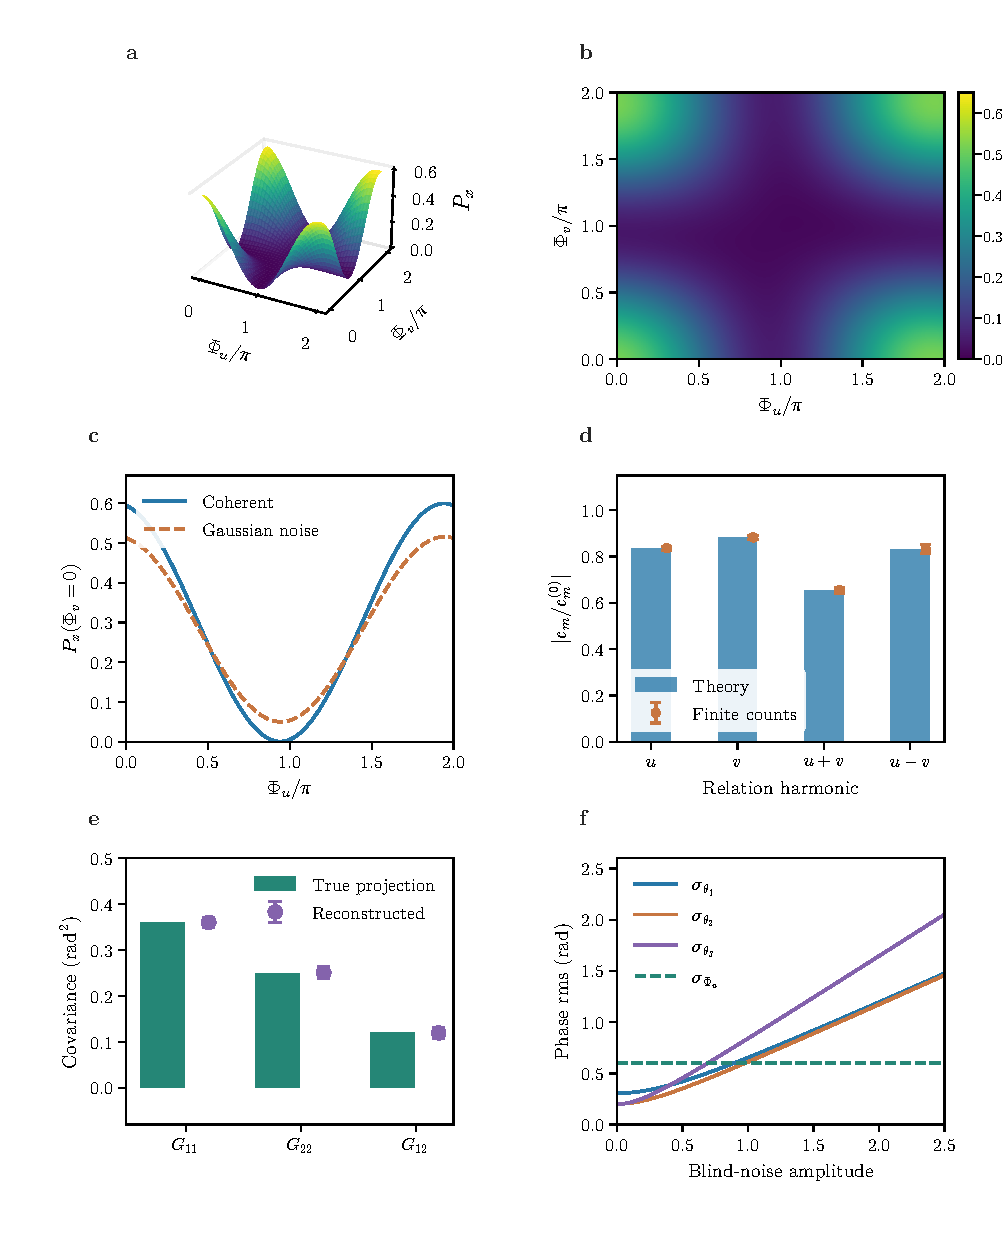
\includegraphics[width=0.96\linewidth,height=0.70\textheight,keepaspectratio]{oam_relation_covariance.pdf}
 \caption{\textbf{由多闭合关系的干涉谐波重建相位噪声投影。} (a) 严格四历史端点模型给出的二维关系相位概率曲面，第三轴是目标端点人口而非真实空间高度；(b) 对相位误差作高斯系综平均后的同一人口；(c) 固定 $\Phi_v=0$ 时的干涉条纹及噪声退相干；(d) 四种关系谐波模长的实测衰减与精确高斯特征函数；(e) 以有限 Bernoulli 计数重建 $G_{11},G_{22},G_{12}$，误差棒是独立重复实验的标准差；(f) 增大关系子空间之外的相位噪声时，单路相位方差不断增长，关系相位却仍保持不变。全部曲线来自同一合法概率模型。}
 \label{fig:oam-relation-covariance}
\end{figure}

这里最容易被误读的地方恰恰是\emph{哪些量不能被重建}。$\Sigma$ 是四路实相位的 $4\times4$ 对称矩阵，一般有 10 个独立数；$G$ 只有 3 个。因此无论端点计数有多精确，同一个 $G$ 都对应许多不同的 $\Sigma$。令 $D=U(U^{\mathsf T}U)^{-1}$，再令矩阵 $Q$ 的列构成 $\ker U^{\mathsf T}$ 的一组正交规范基，就能显式构造整个不可辨识族的一部分：
\begin{equation}
 \Sigma(s)=DGD^{\mathsf T}+s^2QQ^{\mathsf T},\qquad s\ge0,
 \qquad U^{\mathsf T}\Sigma(s)U=G.
 \label{eq:oam-two-loop-blind-family}
\end{equation}
随 $s$ 增大，若干单路相位可以越来越不稳定，但观测到的所有关系谐波完全不变。这个结论是线性代数上的\emph{测量不可辨识性}，而不是对激光稳定性的一般保证，也不表示真实 Maxwell 近场会与额外的噪声完全解耦。

怎样在有限剂量下判断上述反演实际有多精确？假设给定 $K$ 个均匀的关系相位设置，每个设置接收入射电子的二元结果 $Y\in\{x,\varnothing\}$，其成功概率为 $\overline P_x(\Phi_u,\Phi_v;G)$。令 $\vb g=(G_{11},G_{22},G_{12})$，对全部 $K$ 个相位设置平均，\emph{每个入射电子}的 Fisher 信息为
\begin{equation}
 (F_G)_{ab}=\frac1K\sum_{j=1}^{K}
 \frac{(\partial_{g_a}\overline P_x(\boldsymbol\Phi_j))
       (\partial_{g_b}\overline P_x(\boldsymbol\Phi_j))}
 {\overline P_x(\boldsymbol\Phi_j)[1-\overline P_x(\boldsymbol\Phi_j)]}.
 \label{eq:oam-two-loop-fisher}
\end{equation}
所有导数可以对\cref{eq:oam-two-loop-gaussian-filter} 逐项解析求出，例如 $\partial_{G_{11}}\overline c_{\vb m}=-\tfrac12m_1^2\overline c_{\vb m}$、$\partial_{G_{12}}\overline c_{\vb m}=-m_1m_2\overline c_{\vb m}$。若 $N_{\rm e}$ 次独立电子均匀分配到相位设置，总 Fisher 矩阵为 $N_{\rm e}F_G$；在常规局部可辨识和正则条件下，无偏估计量满足 $\operatorname{Cov}(\widehat{\vb g})\succeq(N_{\rm e}F_G)^{-1}$。即使拟合算法形式上以 $\Sigma$ 的 10 个独立分量为未知量，对应 Fisher 矩阵也只能写成 $J^{\mathsf T}F_GJ$，其中 $J=\partial\vb g/\partial\vb\sigma$ 是 $3\times10$ 雅可比矩阵。因此其秩至多为 3，至少七个方向无法由这种端点测量辨认。增加电子剂量可以减小这三个方向的统计误差，却不能使严格为零的信息本征值变正。

\begin{figure}[!htbp]
 \centering
 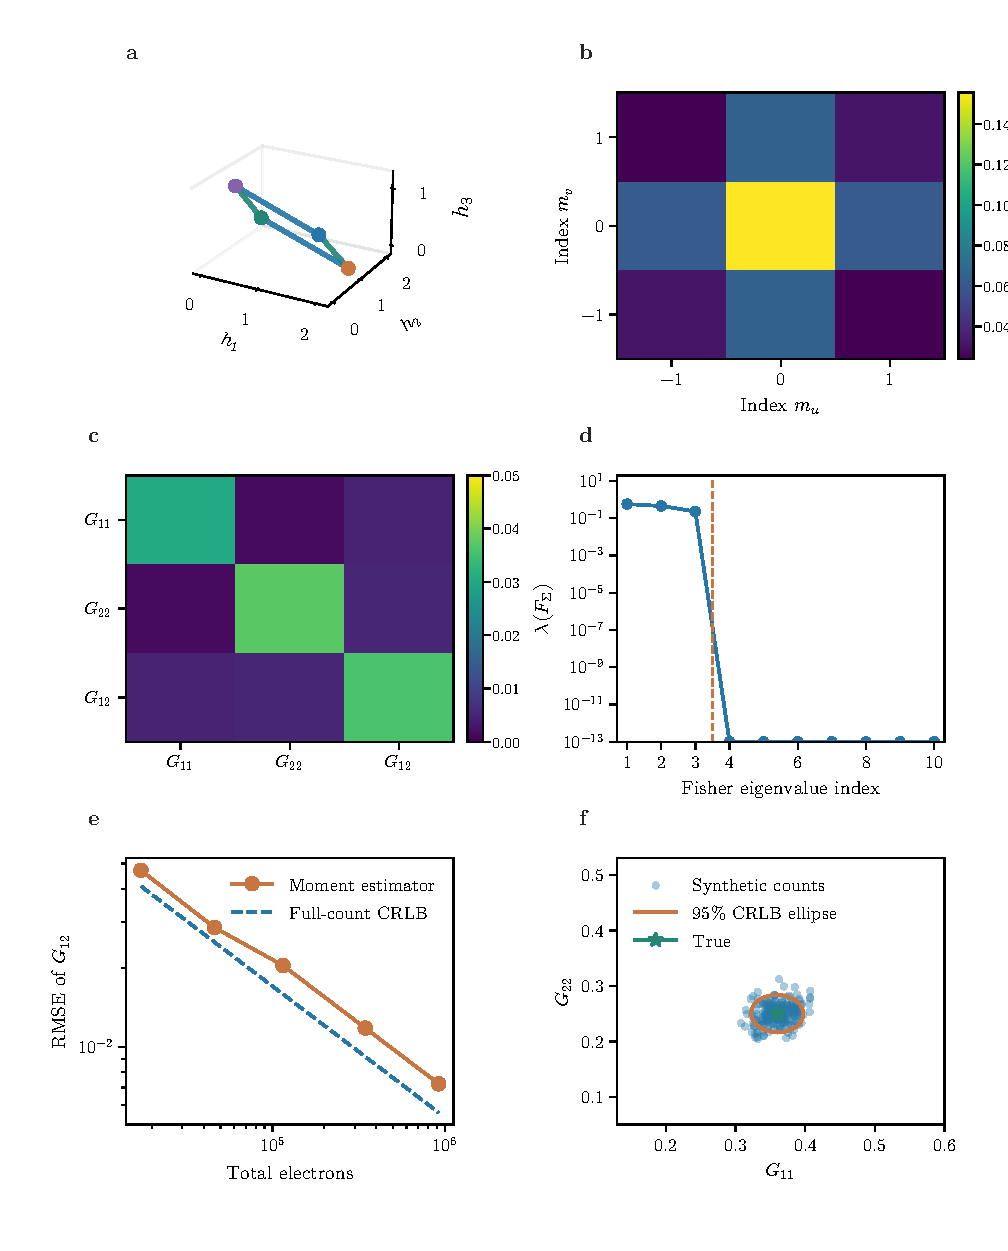
\includegraphics[width=0.96\linewidth,height=0.70\textheight,keepaspectratio]{oam_relation_identifiability.pdf}
 \caption{\textbf{两关系协方差层析的可辨识维度与有限计数。} (a) 四条交换历史在基本事件计数 $(h_1,h_2,h_3)$ 中的投影，它们在完整能量--OAM 端点 $(3,1)$ 上重合；第四事件计数没有作为虚构空间轴；(b) 已平均端点概率的二维关系 Fourier 支撑；(c) 对 $G_{11},G_{22},G_{12}$ 的每电子 Bernoulli Fisher 矩阵；(d) 将其拉回四路相位协方差的十维参数空间，只有三个正信息本征值；(e) 对相关性 $G_{12}$ 作有限计数 Fourier 矩估计，比较重复模拟的均方根误差与完整计数 Cramér--Rao 下界；(f) 有限剂量估计的散点与局域 Fisher 近似给出的二维 $95\%$ 椭圆。第三坐标、色标和置信椭圆都代表指定模型的可观测数学量。}
 \label{fig:oam-relation-identifiability}
\end{figure}

数值计算中，取上面的四条合法整数历史，选 $t_0=0.24,t_u=0.18,t_v=0.16,t_{uv}=0.20\ee^{0.35\ii}$；因此总振幅模不超过 $0.78$，目标端点概率严格小于 $0.609$。关系子空间的真实噪声协方差设为
$G=\begin{psmallmatrix}0.36&0.12\\0.12&0.25\end{psmallmatrix}$，为半正定矩阵。两图的关系相位扫描取 $24\times24$ 个均匀点；第一张的三维面使用 $74\times74$ 点。第一张图 (e) 每点接收 $600$ 个独立 Bernoulli 计数，作 $160$ 次种子为 $2410$ 的重复模拟；图 (f) 用 $s\in[0,2.5]$ 的 $100$ 点扫描\cref{eq:oam-two-loop-blind-family}。第二张图 (b) 的 Fourier 系数由四路径振幅解析求和；图 (c,d) 使用精确导数在 $24\times24$ 相位网格上计算信息矩阵；图 (e) 每相位点电子数取 $30,80,200,600,1600$，各作 $200$ 次独立二项式采样，所示总剂量为单点剂量乘以 $576$；图 (f) 每点 $250$ 个电子、重复 $220$ 次，$95\%$ 椭圆用 $\chi^2_2=5.991$ 的正态近似画出。图像中的 Fourier 矩估计并未声称达到完整计数 Fisher 下界，尤其小样本的非线性对数比估计存在偏差。

这一计算把\emph{共同末态干涉}与\emph{可辨识性层级}放在同一逆问题中，但并不是已有的能量--OAM 实验验证。它增加的是一种有严格可证伪条件的\emph{关系噪声投影层析}：测量前需要先确定哪些复合历史确实能到达同一端点、用参考扫描标定四条复振幅，且证明噪声在每个电子采样时间内近似平稳高斯。如果未来能够找到能激活更多独立关系向量的光学架构，还能逐步扩展可辨识子空间；但没有新增物理读出荷或独立干涉关系，就绝不可能只凭增加图像面板数目恢复完整的四路相位噪声。


角同距性告诉我们，某些角相位纹理在同一个测量设置下无法区分；关系晶格则进一步告诉我们，末态标签是否保留一条历史的信息，会改变哪些相干交叉项能够出现。二者合在一起自然引出一个实验问题：假如双光子 OAM 通道能够揭示某种隐藏角结构，但恰好因为贝塞尔零点或探测效率而没有足够事件，能否改变相互作用的
\emph{读出方式}，让已有信息出现在更容易探测的通道？

一种明确的理论方案是让电子在同一次相干作用中同时经过未知角场和一个可标定的零 OAM 参考场。这里的参考并不是对已测数据施加数学滤波，而是实际改变电子所经历的复相位调制。令未知场为此前六扇区构造的 $s_H(\varphi)$，$H=A,B$，样品无量纲耦合为 $a>0$；让参考具有均匀角相位、实幅度 $r\ge0$ 和受控相位 $\chi$。相干作用区内的总耦合为
\begin{equation}
 \beta_H(\varphi;r,\chi)=a s_H(\varphi)+r\ee^{\ii\chi}.
 \label{eq:oam-coherent-reference-field}
\end{equation}
要求参考场与样品场具有相同的光频，且在电子相互作用窗口内具有可比较的纵向相位匹配与径向包络。若两束光沿电子轨迹的相位不能保持固定，不能使用上式的逐点复数相加。实验上的具体参考近场还需要 Maxwell 模型和相位标定；以下计算只讨论已经满足这些条件的有效耦合。

电子刚离开作用区时，各角度上的第 $n$ 阶振幅仍由完整的贝塞尔形式给出，不过它的\emph{模和相位现在都依赖角度}：
\begin{align}
 c_n^H(\varphi;r,\chi)
 &=J_n\!\left(2|\beta_H(\varphi;r,\chi)|\right)
 \ee^{\ii n\arg[-\beta_H(\varphi;r,\chi)]},\\
 C_{nM}^H(r,\chi)
 &=\frac1{2\pi}\int_0^{2\pi}
 c_n^H(\varphi;r,\chi)\ee^{-\ii M\varphi}\,\dd\varphi,
 \qquad P_{nM}^H=|C_{nM}^H|^2.
 \label{eq:oam-reference-nonlinear-fourier}
\end{align}
取 $r=0$ 时，$|\beta_H|=a$，立刻退回到\cref{eq:oam-homometry-joint}：两场的 $n=1$ OAM 谱严格相同。因此增加参考之后出现的差异，不能错误归因于旧谱本来就包含某个可由数值放大提取的弱峰；参考实际上创造了新的受控干涉测量。

为什么一个\emph{零 OAM}参考可能让一光子边带看到原本只有更高阶才显露的角信息？最清楚的答案来自弱场展开。写 $z=\ee^{\ii\chi}$、$\beta=a s+r z$，使用 $J_1(2x)=x-x^3/2+O(x^5)$，保留到复场幅度三次，有
\begin{align*}
 c_1(\varphi)
 &=-\beta+\tfrac12|\beta|^2\beta+O((a+r)^5),\\
 |\beta|^2\beta
 &=a(a^2+2r^2)s+r(2a^2+r^2)z
   +a^2r z^*s^2+ar^2z^2s^*.
\end{align*}
第一行的线性项只有 $s$ 与角向常数；对于当前 A/B 掩模，$|\widetilde{s_A}_M|^2=|\widetilde{s_B}_M|^2$，并且两场的 $M=0$ Fourier 振幅均为 $2/3$。因此在\emph{严格线性响应近似}中，任何已知均匀参考的强度和相位都不能区分这对场。真正发生变化的是三次项中的 $a^2r z^*s^2$：它把二阶角相位谐波混进了 $n=1$ 的散射振幅。这里展示了与原有高阶边带读出不同的一种可能性：通过相干参考和 PINEM 本身的贝塞尔非线性，将被隐藏的角信息重新编码到较低能量阶。此展开只在 $a+r\ll1$ 时是受控近似；任意强度下的图像和剂量判断必须使用\cref{eq:oam-reference-nonlinear-fourier} 的完整贝塞尔振幅。

这个办法也有特别清楚的适用边界。对于原六扇区掩模，零参考时双光子 OAM 的结构虽然不同，然而选择 $a=a_\star$ 使
\begin{equation}
 J_2(2a_\star)=0,\qquad a_\star\simeq2.567811,
 \label{eq:oam-reference-bessel-zero}
\end{equation}
就使整个无参考 $n=\pm2$ 边带的事件概率严格为零。此时“条件双光子谱很不同”在实验上没有作用，因为根本得不到这个条件事件。把 $r>0$ 代回完整贝塞尔计算后，角向模长不再恒定，原本消失的通道可以重新出现；更有意思的是 $n=1$ 通道也可能开始区分 A/B。这里并不存在克服某个量子信息定理的悖论：改变 $r,\chi$ 改变了输入作用场，已经不再是对原始无参考数据做与样品无关的随机后处理。

为了把这个效应变成可检验的有限剂量预测，不能只画归一化条件 OAM 谱。令实际收集的模为 $M\in\mathcal W$、OAM sorter 的列归一响应为 $K_{MM'}$、成功读出效率为 $0\le\eta_{\rm d}\le1$。对\emph{一个入射电子}，正一阶的已读出概率以及全部未选中事件的概率分别为
\begin{align}
 q^H(M;r,\chi)&=\eta_{\rm d}\sum_{M'\in\mathcal W}
 K_{MM'}|C_{1M'}^H(r,\chi)|^2,
 \qquad M\in\mathcal W,\\
 q^H(\varnothing;r,\chi)&=1-\sum_{M\in\mathcal W}q^H(M;r,\chi).
 \label{eq:oam-reference-detected-events}
\end{align}
第二行把未进入正一阶的电子、未收集的 OAM 尾部以及读出损失合并为一个合法的末态事件；它没有被丢掉或在后选择后悄悄重新归一化。因此每种假设都严格满足 $\sum_{M\in\mathcal W}q^H(M)+q^H(\varnothing)=1$。对两种候选场定义每个入射电子的重叠和判别指数
\begin{equation}
 \Lambda_1(r,\chi)=\sum_{y\in\mathcal W\cup\{\varnothing\}}
 \sqrt{q^A(y;r,\chi)q^B(y;r,\chi)},\qquad
 \Gamma_1(r,\chi)=-\ln\Lambda_1(r,\chi).
 \label{eq:oam-reference-per-electron-rate}
\end{equation}
利用前面\cref{eq:oam-error-bound} 已证明的乘积性质，$N_{\rm e}$ 个独立电子的等先验最佳判别错误率满足 $P_{\rm err}\le\tfrac12\ee^{-N_{\rm e}\Gamma_1}$。参考相位 $\chi$ 和幅度 $r$ 现在都是测量设计参数，而不是未知材料参数；若它们本身漂移，必须把漂移加入联合前向模型，不能直接引用这里的理想误差上界。

\begin{figure}[!htbp]
 \centering
 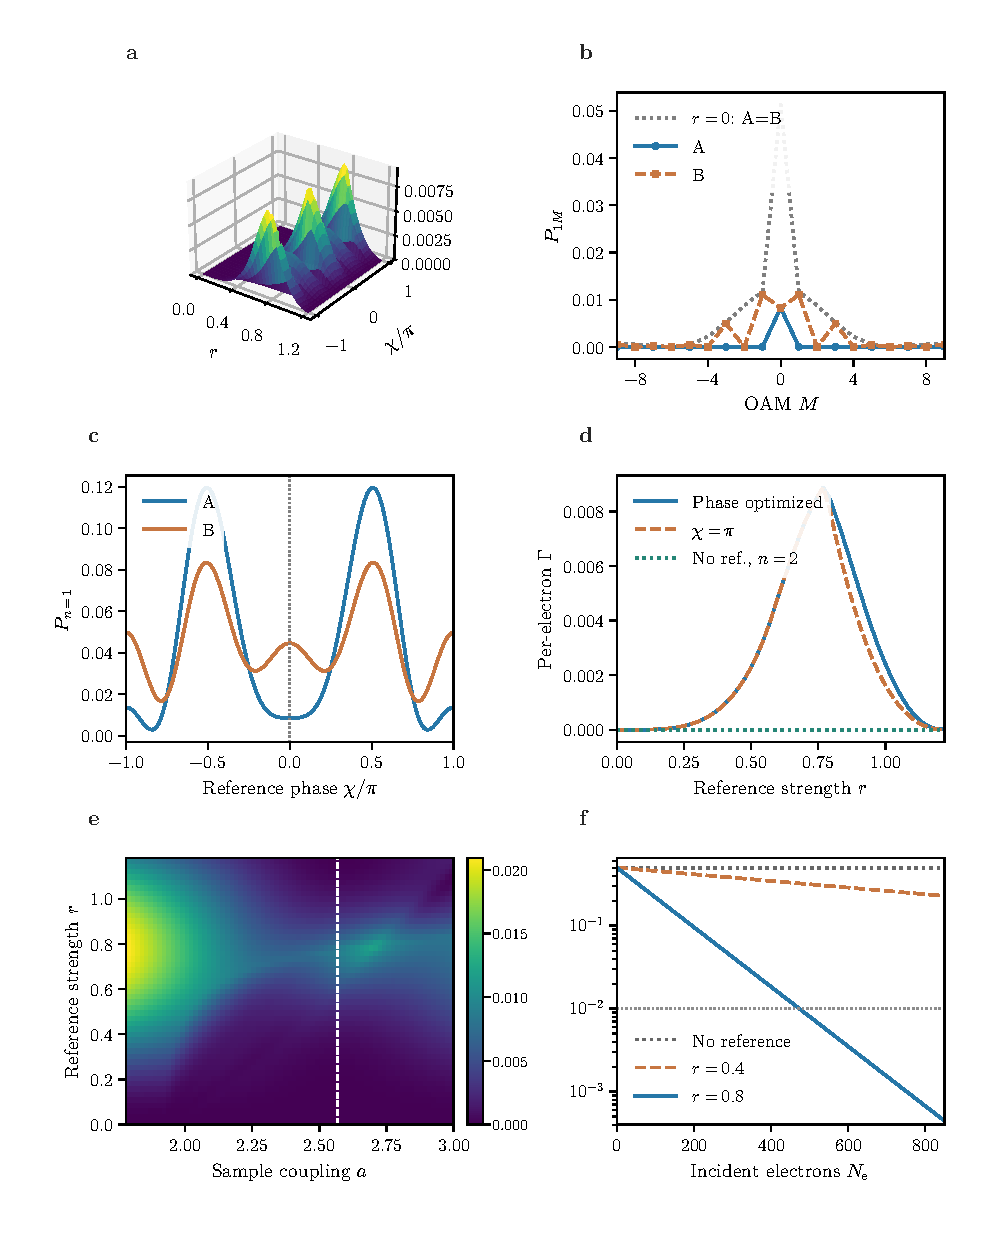
\includegraphics[width=0.96\linewidth,height=0.70\textheight,keepaspectratio]{oam_reference_rescue.pdf}
 \caption{\textbf{相干参考把高阶角信息转入低阶 PINEM 读出的理论延伸。} (a) 在 $J_2$ 零点的样品耦合下，三维曲面显示已计入效率和漏检记录的每入射电子判别指数 $\Gamma_1(r,\chi)$，竖轴不是新的合成空间维度；(b) 比较无参考时重合的一光子 OAM 谱与加入参考后分开的两种联合谱；(c) 参考相位扫描后的正一阶\emph{能量边际}概率，此时已改变物理驱动，不能再套用无参考的能量盲区；(d) 相位优化与固定相位下的一光子判别指数，并对比无参考双光子在贝塞尔零点处的信息为零；(e) 在样品强度和参考强度平面中，用真实的逐通道计数重叠计算 $\Gamma_1$；(f) 比较参考关闭、弱参考和中等参考下的有限剂量错误率\emph{上界}。所有曲线均属于同一相位标定、相同径向包络假设下的有效模型预测。}
 \label{fig:oam-reference-rescue}
\end{figure}

所有面板由\cref{eq:oam-coherent-reference-field,eq:oam-reference-nonlinear-fourier,eq:oam-reference-detected-events,eq:oam-reference-per-electron-rate} 同一前向模型生成。样品掩模采用\cref{eq:oam-six-sector-masks} 的 A/B 六扇区，每扇区宽 $\pi/3$，初始电子角波函数为 $1/\sqrt{2\pi}$；参考场的角向拓扑荷为零，强度 $r$ 为无量纲幅值。第 $n$ 阶每个扇区的振幅为
\[
 f^H_{nj}(a,r,\chi)=J_n(2|a s^H_j+r\ee^{\ii\chi}|)\ee^{\ii n\arg[-a s^H_j-r\ee^{\ii\chi}]},\qquad
 C_{nM}^H=\frac{\operatorname{sinc}(M\pi/6)}6
 \sum_{j=0}^{5}f^H_{nj}\ee^{-\ii M(2j+1)\pi/6}.
\]
所有图只收集 $n=+1$，$M=-12,-11,\ldots,12$；对这些已收集的 OAM 模施加 FWHM 为 $1.1\hbar$ 的离散高斯响应，响应矩阵各列在这个收集窗口内归一化。成功探测效率设为 $\eta_{\rm d}=0.72$，其余事件全部放进一个 ``未选中'' 结果，不做成功事件的条件归一化。此为理想标定的固定效率模型，不含暗计数、背景、材料损耗或参考相位抖动。耦合选在 $a_\star=j_{2,1}/2=2.5678111509$，其中 $j_{2,1}$ 是 $J_2$ 的首个正零点。
(a) 参考幅值 $r\in[0,1.2]$ 取 36 点、$\chi\in[-\pi,\pi]$ 取 61 点，三维高度为 $\Gamma_1$；观察角 $(27^\circ,-54^\circ)$ 不进入数据计算。(b) 在 $M=-9,\ldots,9$ 画理想未展宽的 $|C_{1M}|^2$，比较 $r=0$ 与 $r=0.8$、后者选择 (a) 网格上使 $\Gamma_1$ 最大的相位 $\chi=0$；无参考曲线两场严格重合。(c) 固定 $r=0.8$，以 111 个参考相位计算总能量边际 $P_1^H=\tfrac16\sum_j|f^H_{1j}|^2$。(d) 取 55 个 $r\in[0,1.22]$ 点；蓝线对每个 $r$ 在 31 个 $\chi$ 上最大化 $\Gamma_1$，橙线固定 $\chi=\pi$，水平绿线计算 $r=0,n=2$ 的同一单边带检测模型。(e) 取 $a\in[1.78,3.00]$ 的 73 点、$r\in[0,1.18]$ 的 49 点，固定 $\chi=\pi$ 画 $\Gamma_1$，竖虚线标出 $a_\star$。(f) 入射电子数取 $N_{\rm e}=0,\ldots,849$，对 $r=0,0.4,0.8$ 各自在 61 个 $\chi$ 中选择最大 $\Gamma_1$，画 $\tfrac12\exp(-N_{\rm e}\Gamma_1)$；横线为 $0.01$。在 $a=a_\star,r=0.8$，网格最优相位为 $0$，$\Gamma_1\simeq0.0082654$，使该错误率上界低于 $1\%$ 的充分入射电子数是 $474$；它既不是实测误码率也不计入独立准备参考场的代价。


参考辅助读出并不总是比无参考的高阶读出节省剂量。在相同的 $\eta_{\rm d}=0.72$、$1.1\hbar$ OAM 模糊和 $|M|\le12$ 收集窗口下，把样品耦合改为 $a=0.8$，无参考正二阶的每电子判别指数约为 $0.0276$，而 $r=0.8$ 并优化参考相位后的正一阶只有约 $0.0155$。前者此时更有效；只有当某个高阶边带因贝塞尔零点受到抑制、或仪器无法分辨该阶时，参考辅助读出才可能成为更好的选择。这个比较固定了每个入射电子的概率模型，但还没有计入产生稳定参考场所需的光学资源，不能据此宣称普适的量子增强。

这项延伸也说明如何把两个原本分开的研究思路用于同一个实验设计任务。角同距层级决定\emph{不加参考时何种角信息被隐藏}，而端点关系晶格说明\emph{加参考、增加驱动事件或保留新的末态荷以后，哪条历史差才会产生可见干涉}。在三驱动端点模型中，关系向量 $(1,1,-1)$ 的相位就是 $\theta_1+\theta_2-\theta_3$；在角掩模模型中，参考相位 $\chi$ 则通过\cref{eq:oam-reference-nonlinear-fourier} 改变整个非线性 Fourier 系数。这两个相位旋钮分别作用于事件关系和角向散射，并不代表同一个拓扑不变量。两者若要同时加入真实电子显微镜，必须先用具体 Maxwell 场和相干参考作用区标定跃迁振幅，再以联合 $(n,M)$ 探测器响应计算最优剂量。由于参考可能引入额外漂移与电子辐照负担，不存在对所有耦合、材料和检测条件都最优的单一测量方案。


等能线重连与拓扑相变是两件事。Lifshitz 转变发生在等能线穿过鞍点时，表现为连通方式和态密度改变；Chern 数改变则要求能隙闭合再打开，并伴随 Berry 曲率总积分发生整数变化。比较两者时，必须分别看色散几何和能带本征态，不能只凭一张等能线判断拓扑。


\begin{figure}[!htbp]
\centering
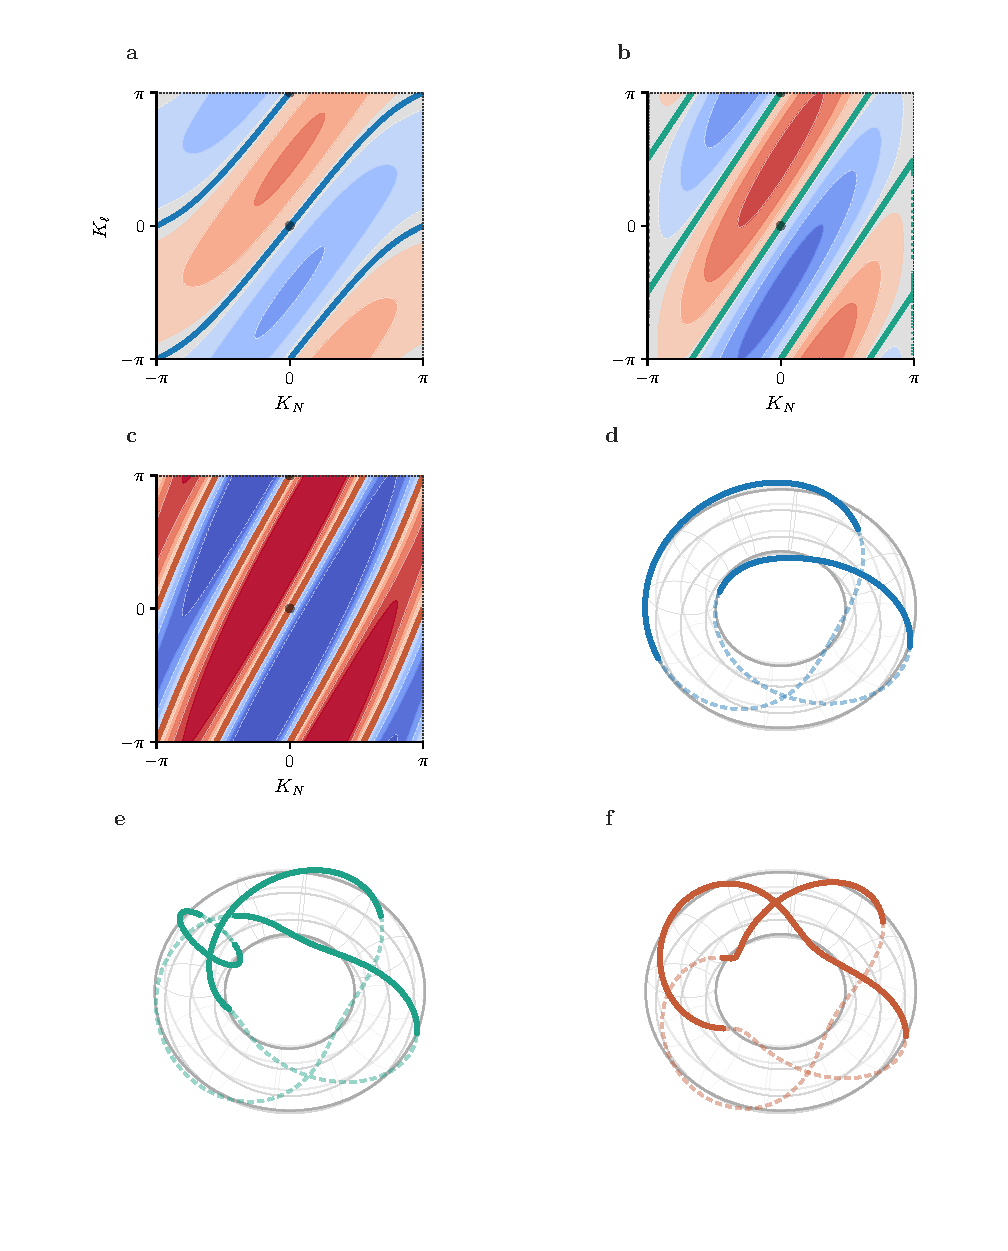
\includegraphics[width=0.96\linewidth,height=0.70\textheight,keepaspectratio]{lifshitz_context.pdf}
\caption{\textbf{Lifshitz 转变的能带几何}\quad 同一双频合成晶格的零准能线在 $|\beta_2/\beta_1|=1/3,1,3$ 时经历从分离口袋到临界颈部再到重连片层的几何变化。上排不只画零能线本身，还用完整准能带等值纹理标出它所处的局域色散背景，因此读者可以直接看出重连发生在鞍点附近。下排把同一条零能线提升到布里渊区环面，并以实线/虚线区分前景与背面，从而消除普通三维绘图里常见的遮挡歧义。这样图像传达的是“周期边界上的真实连通性”，而不是任意视角下的装饰性环面。}
\label{fig:ch03-supporting-theory--01-lifshitz-context}
\end{figure}

具体到各面板，(a,b,c) 对 $\eta=1/3,1,3$ 分别以 $401^2$ 点求 $-2\sin(K_N-K_\ell)-2\eta\sin(2K_N-K_\ell)$ 的符号区及零线，绘图方形有周期边界；(d,e,f) 从对应 (a,b,c) 的\emph{同一条}零线坐标段映入 $R=2.05$、$r=0.66$ 的环面，曲线显示半径增加 $0.085$ 仅为了防遮挡。透明度 $0.085$，辅助经纬线各取 9 个周期角，视角 $(66^\circ,-56^\circ)$；几何可视化不参与能带计算。


若正向和反向跃迁不再互为共轭，或格点存在有效增益与损耗，哈密顿量变成非厄米矩阵，本征值一般进入复平面。这时应使用点隙、线隙和复谱绕数描述谱结构。增加更多独立跃迁向量则可扩展合成维数；这里增加的是状态空间坐标，不是实际空间维数。

取两条线性无关的合成晶格跃迁 $\vb a_1=(1,0)$ 和 $\vb a_2=(1,1)$，无量纲跃迁幅度分别为 $t_1,t_2>0$，并令第二条跃迁带相位 $\phi$。按照\cref{eq:ch03-li-heff} 的构造，令 $\vb k=(k_E,k_\ell)$，对整数格点作 Fourier 变换；由于平移算符在 $|\vb k\rangle$ 上给出本征值 $\ee^{\ii\vb k\cdot\vb a_j}$，本征值相加得到


\begin{equation*}
\varepsilon(k_E,k_\ell)=2t_1\cos k_E+2t_2\cos(k_E+k_\ell+\phi).
\end{equation*}


现在可以直接读出三个控制量。$t_2/t_1$ 决定两条跃迁对带宽和曲率的相对贡献；$\phi$ 平移第二项的相位，因此能移动鞍点和等能线重连位置；$k_E,k_\ell$ 则只是合成准动量坐标。后面的 Lifshitz 参数图就是连续改变 $t_2/t_1$ 与 $\phi$，再检查 $\nabla_{\vb{k}}\varepsilon=0$ 的驻点怎样移动。

这个单带模型的归一本征矢可以选为动量无关的常数，因此 Berry 联络为纯规范项，曲率积分为零。非零 Chern 数需要在布里渊区上不能整体选取同一光滑周期本征基的能带结构；这需要引入内部自由度，而不是仅调节上述两项余弦的参数。

连续改变耦合比和相对相位，可以判断能带结构在哪些参数处发生定性变化。耦合比主要改变色散曲率和鞍点位置，对于平移不变的两条跃迁，常数相位仅平移准动量，不会单独产生不可消除的回路磁通；要研究磁通，必须另外建立有位置依赖相位的闭合晶格回路。


局域规范变换还能判别何种光学相位在晶格上有可观测意义。对\cref{eq:ch03-li-heff} 中两条线性无关、平移不变的跃迁，两个常数相位可通过给格点重新赋相位而消去；因此单靠两束光的相对相位，不能在该无限晶格上生成均匀合成磁场。不可消去的磁通必须定义在某条闭合回路上：沿回路跃迁振幅的相位积累之和为
\begin{equation}
 \Phi_{\square}=\arg\!\prod_{\langle ij\rangle\in\partial\square} t_{ji},
 \label{eq:ch03-loop-flux}
\end{equation}
其中乘积依给定方向绕行。它在格点局域相位变换 $|j\rangle\mapsto \ee^{\ii\chi_j}|j\rangle$ 下不变。要把这种回路磁通落实到实际能量--OAM 合成晶格，必须进一步设计格点依赖的驱动相位、辅助耦合通道或多步回路；这超出了前面只含均匀双频跃迁的最小 PINEM 模型。

一个适合作为理论延伸的最小基准是方形 Harper--Hofstadter 格子。它不声称已经在前述 PINEM 实验中实现，而是用可控制的 Peierls 相位测试磁通、边缘谱和波包的关系：
\begin{equation}
 H_{\mathrm H}=-\sum_{x,y}\bigl[t_xe^{\ii2\pi\alpha y}|x{+}1,y\rangle\langle x,y|
 +t_y|x,y{+}1\rangle\langle x,y|+\mathrm{h.c.}\bigr],
 \quad \Phi_{\square}=\pm2\pi\alpha .
 \label{eq:ch03-hofstadter}
\end{equation}
符号取决于回路方向。沿 $x$ 保持 Bloch 平移、沿 $y$ 开边界时，它化为一维 Harper 条带矩阵，具有对角元 $-2t_x\cos(k_x+2\pi\alpha y)$ 以及相邻 $y$ 之间的跃迁 $-t_y$。图中先扫描磁通与能带，再用开边界条带寻找位于体能隙中的边界模，最后对一个从边界附近发射的有限宽度波包直接演化。后者会同时激发边界态和体态，所以“边缘几行保留的概率”只能作为动力学诊断，不能单独当作边缘态拓扑保护的证明。

\begin{figure}[!htbp]
\centering
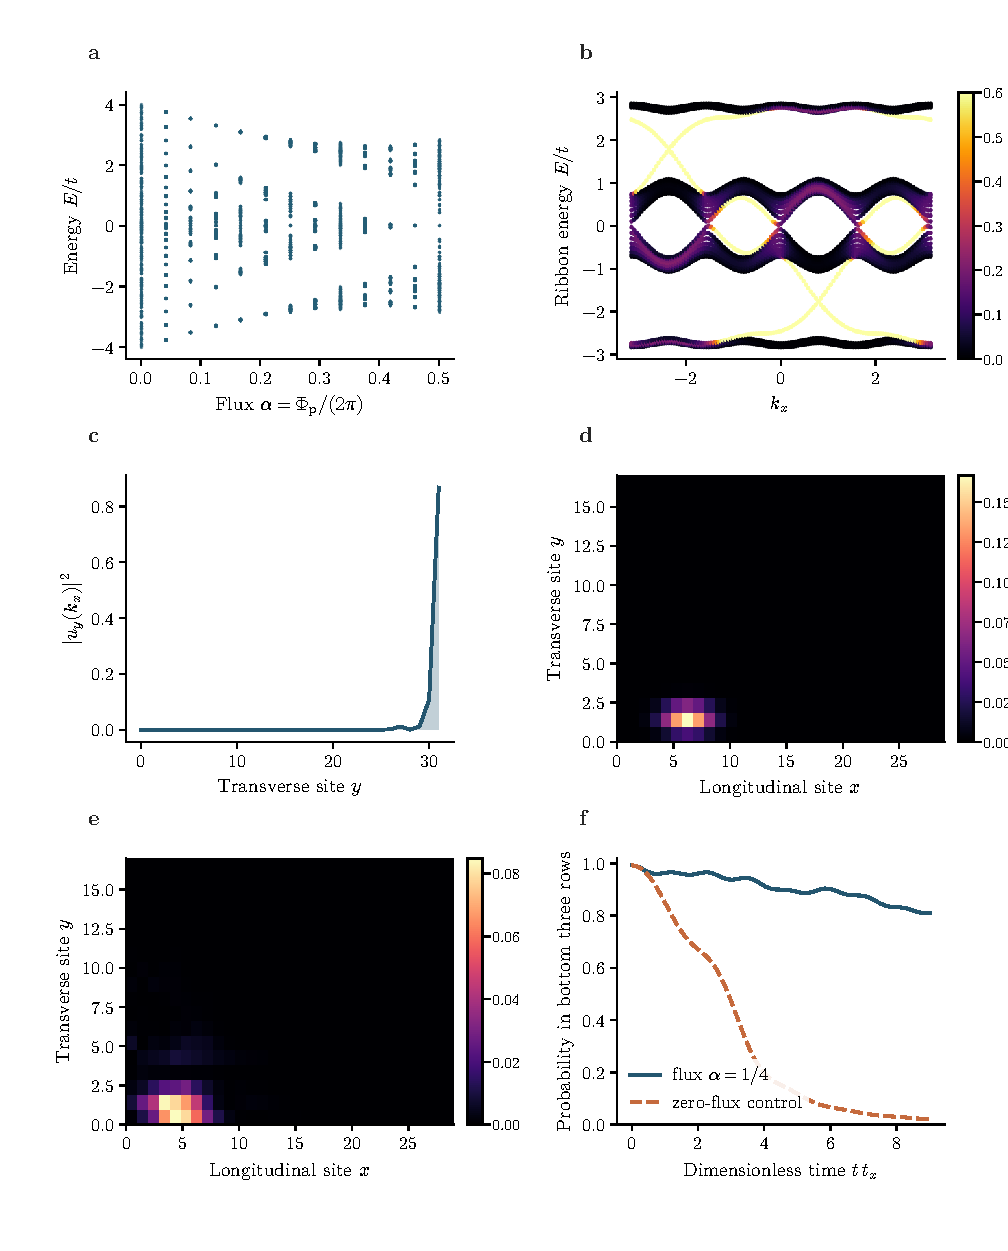
\includegraphics[width=0.96\linewidth,height=0.70\textheight,keepaspectratio]{synthetic_magnetic_flux.pdf}
\caption{\textbf{合成磁通的谱学与传播诊断。} (a) 在周期横向边界的固定扭转角截面上扫描有理磁通 $\alpha=p/24$，计算磁性子带；(b) 对 $\alpha=1/4$ 的开边界条带计算能谱，颜色为本征态在两侧边缘的概率权重；(c) 直接画一个边缘权重较大本征态的横向密度，检验它是否实际局域；(d,e) 将同一边缘高斯初态投入有限二维格点，比较传播前后强度分布；(f) 将含磁通和零磁通两种哈密顿量作用于相同初态，比较边缘三行的概率保留。六格使用同一种厄米最近邻耦合，没有添加隐藏的非厄米损耗项。}
\label{fig:ch03-synthetic-flux-dynamics}
\end{figure}

六个面板均由\cref{eq:ch03-hofstadter} 的厄米最近邻模型计算，取 $t_x=t_y=1$，不加入势能、无序、退相干或损耗。对 (a)，使用 $\alpha=p/24$、$p=0,\ldots,12$，每个磁通取 $28$ 个 $k_x\in[-\pi,\pi)$，横向 $24$ 格点采取周期边界且固定 $k_y=0$ 的扭转；它是二维磁能带在固定扭转角上的截面，不是对所有 $k_y$ 积分得到的完整谱密度。(b,c) 固定 $\alpha=1/4$，条带宽 $N_y=32$、$k_x\in[-\pi,\pi]$ 均匀取 $121$ 点；(b) 的颜色取最上端和最下端各两个格点的总权重，(c) 从 $0.15<|E|<1.75$ 的候选态中取边界权重最大的本征矢，并归一化为 $\sum_y|u_y|^2=1$。(d,e) 使用沿 $x,y$ 均开边界的 $N_x\times N_y=30\times18$ 格点，初态严格取
\[
 \psi_{xy}(0)=\mathcal N\exp\!\left[-\frac{(x-6)^2}{2(2.1)^2}-\frac{(y-1.1)^2}{2(0.9)^2}+\ii(0.75)x\right],
 \quad\sum_{x,y}|\psi_{xy}|^2=1,
\]
以 $\psi(t)=\ee^{-\ii H_{\rm H}t}\psi(0)$ 在 $t\in[0,9]$ 取 $75$ 个时间点；(d) 为 $t=0$，(e) 为离散采样最接近 $t=7.2$ 的波包概率 $|\psi_{xy}(t)|^2$，两格各自使用绝对概率色标（色标最大值分别取该时刻最大格点概率），不可直接比较视觉亮度。(f) 对同一初态和相同开边界条件分别取 $\alpha=1/4$ 与 $\alpha=0$，计算 $P_{\rm edge}(t)=\sum_{y=0}^{2}\sum_x|\psi_{xy}(t)|^2$。整个模型只用于说明新增位置依赖相位以后有哪些可复现的谱学和波包诊断，不把此处的格点长度或耦合标定成真实电子实验单位。


单带色散只有一个标量本征值，没有随动量旋转的内部自旋量。若要让能带本征态本身携带几何信息，可在每个晶格准动量处引入两分量内部基底，并写出
\begin{equation}
 H(\vb k)=d_0(\vb k)\mathbb I+\vb d(\vb k)\cdot\boldsymbol\sigma ,
 \qquad |\vb d(\vb k)|>0.
 \label{eq:ch03-4}
\end{equation}
这里 $\boldsymbol\sigma=(\sigma_x,\sigma_y,\sigma_z)$ 是 Pauli 矩阵，$\vb d$ 为实三维向量；条件 $|\vb d|>0$ 保证两个能带分离。利用 $(\hat{\vb d}\cdot\boldsymbol\sigma)^2=\mathbb I$，下能带的谱投影为 $P_-=(\mathbb I-\hat{\vb d}\cdot\boldsymbol\sigma)/2$。取联络约定 $\mathcal A_\mu=-\ii\langle u_-|\partial_\mu u_-\rangle$，曲率可由不依赖本征矢相位的投影算符计算：
\begin{align*}
 \Omega_{xy}&=-\ii\operatorname{Tr}\!\left(P_-[\partial_{k_x}P_-,\partial_{k_y}P_-]\right),\\
 [\partial_{k_x}P_-,\partial_{k_y}P_-]
 &=\frac14[\partial_{k_x}\hat{\vb d}\cdot\boldsymbol\sigma,
 \partial_{k_y}\hat{\vb d}\cdot\boldsymbol\sigma]\\
 &=\frac{\ii}{2}\bigl(\partial_{k_x}\hat{\vb d}\times\partial_{k_y}\hat{\vb d}\bigr)\cdot\boldsymbol\sigma.
\end{align*}
其中第二行使用了 $[\vb a\cdot\boldsymbol\sigma,\vb b\cdot\boldsymbol\sigma]=2\ii(\vb a\times\vb b)\cdot\boldsymbol\sigma$。再用 $\operatorname{Tr}(\sigma_i\sigma_j)=2\delta_{ij}$，便得到
\begin{equation}
 \Omega_{xy}=-\frac12\hat{\vb d}\cdot
 \bigl(\partial_{k_x}\hat{\vb d}\times\partial_{k_y}\hat{\vb d}\bigr),\qquad
 C=\frac{1}{2\pi}\int_{\mathrm{BZ}}\Omega_{xy}\,\dd^2k.
 \label{eq:ch03-5}
\end{equation}
当能隙处处不为零时，$C$ 是整数；改变它必须经过能隙闭合。Wilson 环沿闭合准动量路径累计同一联络，条带边缘谱则用于检验由体能带拓扑预言的边界模。


\begin{figure}[!htbp]
\centering
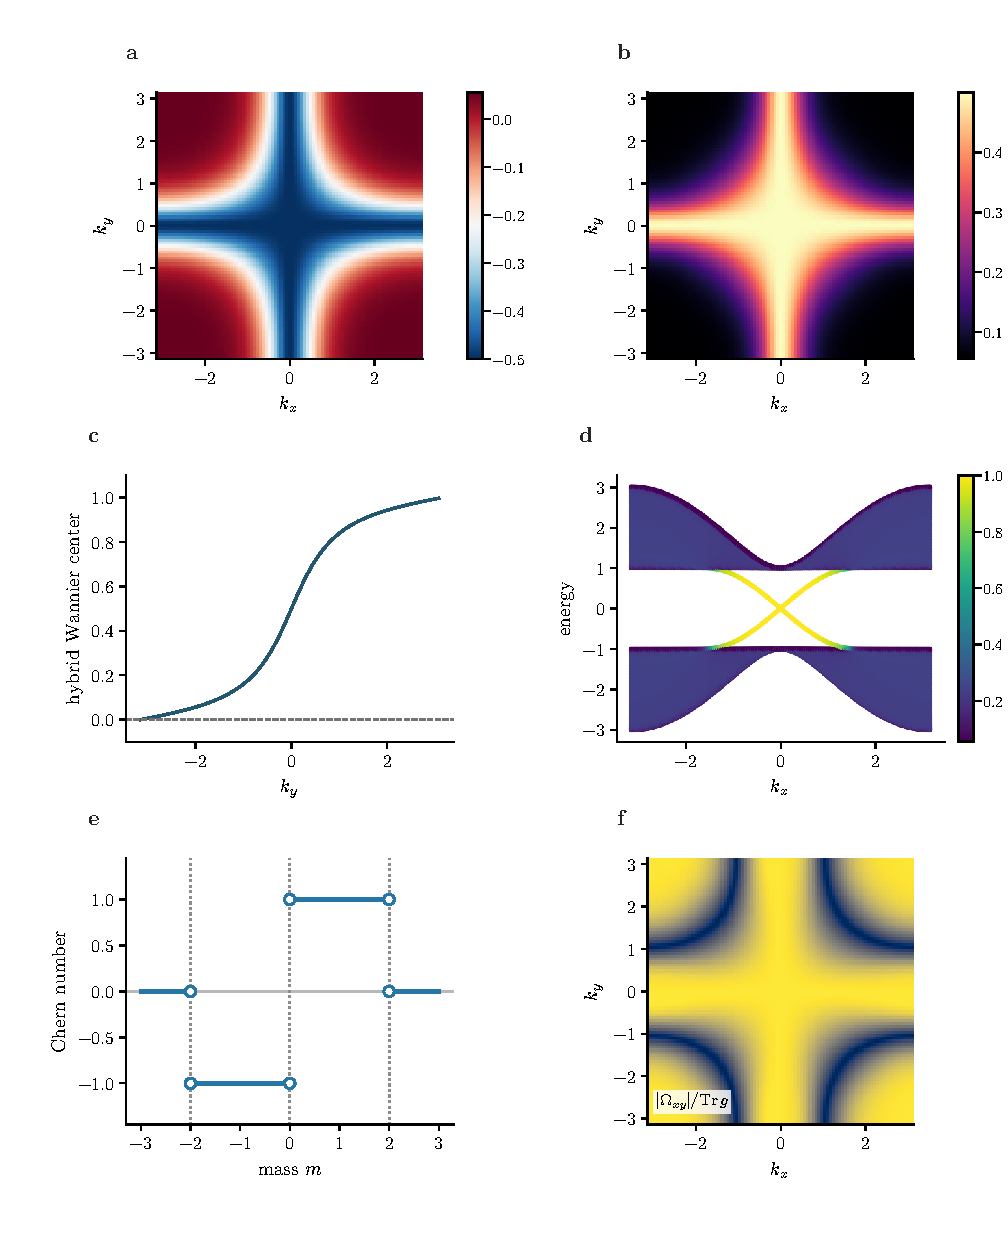
\includegraphics[width=0.96\linewidth,height=0.70\textheight,keepaspectratio]{quantum_geometry_wilson_loops.pdf}
\caption{\textbf{量子几何、Wilson 环与条带边缘态的一致检验}\quad 采用两带 Qi--Wu--Zhang 模型 $H(\vb k)=\sin k_x\,\sigma_x+\sin k_y\,\sigma_y+(m+\cos k_x+\cos k_y)\sigma_z$，在拓扑区 $m=-1$ 同时计算 Berry 曲率、Fubini--Study 量子度规、Wilson 环流与开边界条带谱。上排显示局域几何：Berry 曲率在带隙闭合邻域集中，量子度规在临界线附近增强，Wilson 环出现绕行，对应一条混合 Wannier 中心跨越一个晶格周期。下排显示边界与参数扫描：条带谱中跨隙色散的边缘支与非零 Chern 数对应，Chern 数在 $m=0,\pm2$ 的闭隙处发生跳变。最后一格给出局域比值 $|\Omega_{xy}|/\operatorname{Tr}\,g$，用于并列比较拓扑曲率与量子度规的空间分布。}
\label{fig:ch03-novel-extensions--12-quantum-geometry-wilson-loops}
\end{figure}

采用 Qi--Wu--Zhang 两带模型
\[H(\vb k)=\sin k_x\,\sigma_x+\sin k_y\,\sigma_y+(m+\cos k_x+\cos k_y)\sigma_z,\quad m=-1.\]
主图上排使用 $k_x,k_y\in[-\pi,\pi)$ 的 $91\times91$ 均匀网格；Berry 曲率由规范不变格点 Wilson 余角
\[\Omega_{xy}(\vb k)\approx \frac{1}{\Delta k^2}\arg\Bigl(U_x(\vb k)U_y(\vb k+\hat x)U_x(\vb k+\hat y)^{-1}U_y(\vb k)^{-1}\Bigr),\qquad U_\mu(\vb k)=\frac{\langle u(\vb k)|u(\vb k+\hat\mu)\rangle}{|\langle u(\vb k)|u(\vb k+\hat\mu)\rangle|},\]
量子度规迹由最近邻重叠估计 $g_{xx}\approx[1-|\langle u|u_{x}\rangle|^2]/\Delta k^2$、$g_{yy}\approx[1-|\langle u|u_{y}\rangle|^2]/\Delta k^2$。Wilson 环沿 $k_x$ 方向相乘规范化重叠，输出混合 Wannier 中心 $\nu(k_y)=\arg\prod_{k_x}U_x(k_x,k_y)/(2\pi)$，再做相位展开。条带谱采用 $N_y=42$ 条链、沿 $y$ 开边界、沿 $x$ 保持 Bloch 动量；边缘权重对两端按 $e^{-y/4}$ 加权。计算中 Chern 数和度规体积分别定义为
\[C=\frac{1}{2\pi}\int_{\mathrm{BZ}}\Omega_{xy}\,\dd^2 k,\qquad \mathcal G=\frac{1}{(2\pi)^2}\int_{\mathrm{BZ}}\operatorname{Tr}g\,\dd^2 k,\]
质量扫描覆盖 $m\in[-3,3]$；面板 (e) 的 Chern 数取解析分段结果，闭隙点用空心标记表示该数值无定义。直接带隙可精确求得为
\begin{equation*}
 \Delta(m)=2\min\{|m+2|,|m|,|m-2|\}.
\end{equation*}
因为令 $u=\cos k_x,v=\cos k_y$ 后，$|\vb d|^2=2-u^2-v^2+(m+u+v)^2$ 在固定另一个变量时分别对 $u$、$v$ 呈线性，最小值必落在 $u,v\in\{-1,1\}$。因此 $m=-2,0,2$ 是全部可能的闭隙点。

这三个参数为何伴随整数跃迁，可以直接从闭隙处的局域色散算出。在动量 $\vb k_\star$ 的邻域令 $\vb k=\vb k_\star+\vb q$，记
\[
 v_x=\cos k_{\star x},\qquad v_y=\cos k_{\star y},\qquad
 M=m+\cos k_{\star x}+\cos k_{\star y}.
\]
原来的两带哈密顿量到一阶成为
\[
 H(\vb k_\star+\vb q)=v_xq_x\sigma_x+v_yq_y\sigma_y+M\sigma_z+O(|\vb q|^2).
\]
将这个表达式代入下带 Berry 曲率公式，得到
\begin{align*}
 \Omega_{xy}(\vb q)
 &=-\frac{Mv_xv_y}{2(v_x^2q_x^2+v_y^2q_y^2+M^2)^{3/2}},\\
 \frac1{2\pi}\int_{\RR^2}\Omega_{xy}(\vb q)\,\dd^2q
 &=-\frac12\operatorname{sgn}(v_xv_y)\operatorname{sgn}M.
\end{align*}
积分中先代换 $p_x=|v_x|q_x$、$p_y=|v_y|q_y$，再用极坐标积分
$\int_0^\infty r\,\dd r/(r^2+M^2)^{3/2}=1/|M|$。
在质量趋近零的局域极限，每个锥的半整数贡献确定其质量变号时 Chern 数的整数跳跃。
四个闭隙动量 $(0,0),(\pi,0),(0,\pi),(\pi,\pi)$
分别具有手性 $\operatorname{sgn}(v_xv_y)=+1,-1,-1,+1$，
质量分别是 $m+2,m,m,m-2$。
从 $m>2$ 时可连续缩成常向量的平庸相 $C=0$ 出发，逐一计入各个质量变号，得到整个格点模型的精确分段结果
\begin{equation}
 C(m)=-\frac12\bigl[\operatorname{sgn}(m+2)-2\operatorname{sgn}(m)+\operatorname{sgn}(m-2)\bigr],\qquad m\notin\{-2,0,2\}.
 \label{eq:qwz-chern-phase}
\end{equation}
于是 $-2<m<0$ 时 $C=-1$，$0<m<2$ 时 $C=1$，其余有隙区间 $C=0$；
在闭隙参数处，下带投影不能在整个布里渊区连续定义，单带 Chern 数无定义。

最后一格绘制比值 $|\Omega_{xy}|/(\operatorname{Tr}g+10^{-12})$，以统一色标展示该无量纲几何比值；它不是新的拓扑不变量。


局域 Berry 曲率积分后得到 Chern 数，沿布里渊区绕行的 Wilson 环则将相同几何信息写成混合 Wannier 中心的位移。当这一整数不为零，适当开边界的条带谱可以出现跨越体带隙的手性边界模。三者共同构成对厄米能带拓扑的不同检验；单独出现一处曲率峰并不足以证明非平凡拓扑。

\begin{figure}[!htbp]
\centering
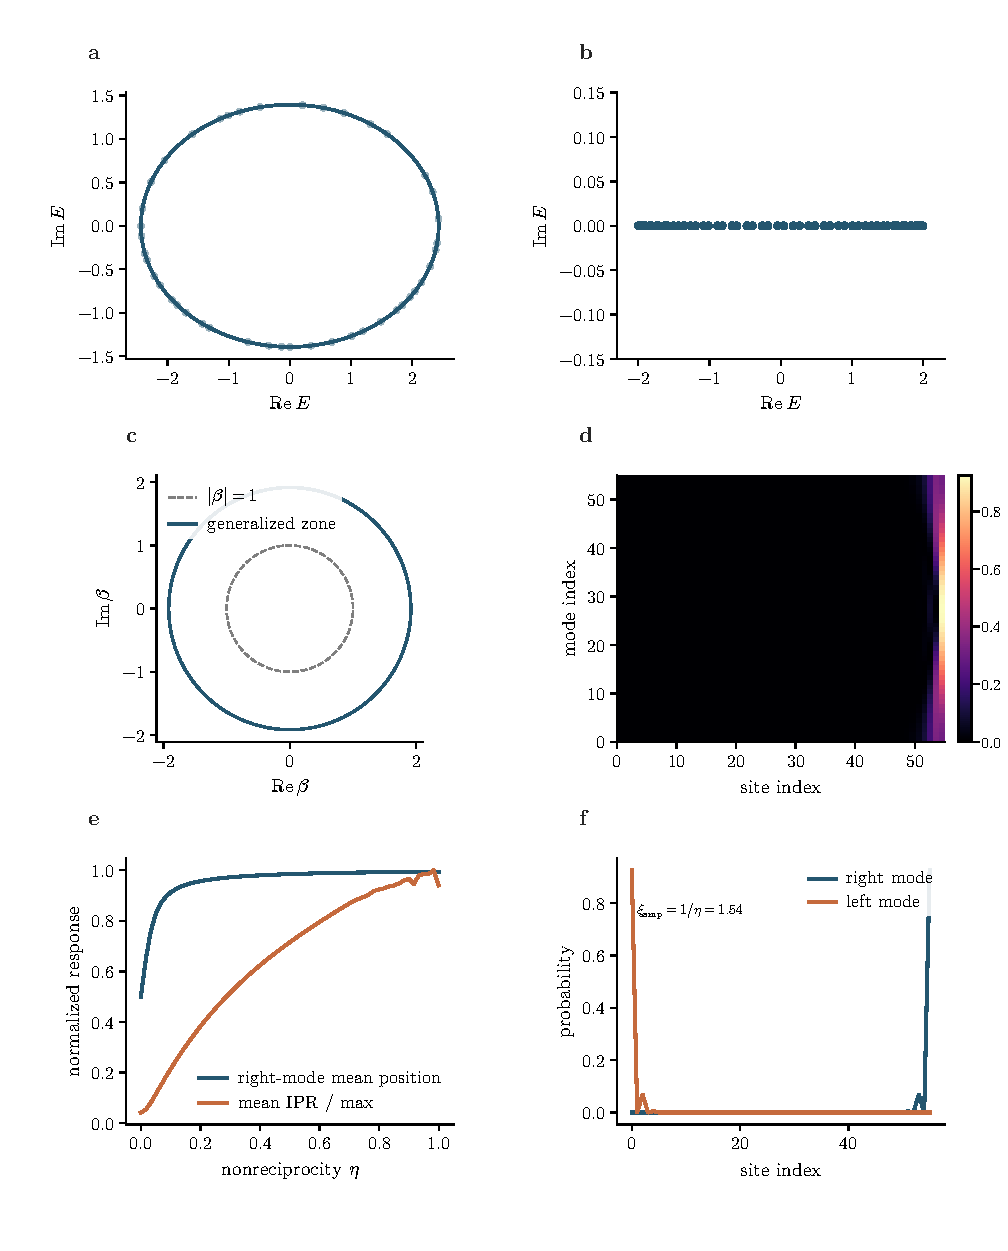
\includegraphics[width=0.96\linewidth,height=0.70\textheight,keepaspectratio]{nonhermitian_skin_topology.pdf}
\caption{\textbf{非厄米合成链中的趋肤谱与广义布里渊区}\quad 以非互易 Hatano--Nelson 链 $H=\sum_n(t_R|n{+}1\rangle\langle n|+t_L|n\rangle\langle n{+}1|)$，其中 $t_R=t e^{\eta},t_L=t e^{-\eta}$，比较周期边界与开边界复谱。周期边界下本征值形成复能量点隙环；开边界下谱塌缩到皮肤谱线，右本征模集体堆积到一侧边界。第三格按 $\psi_j\propto\beta^j$ 的约定给出广义布里渊区 $|\beta|=\sqrt{|t_R/t_L|}$，说明非布洛赫波矢才与开边界谱一致；后两格再用平均 IPR、边界权重以及左右本征态轮廓量化趋肤局域。}
\label{fig:ch03-novel-extensions--07-nonhermitian-skin-topology}
\end{figure}

采用非互易 Hatano--Nelson 链
\[H=\sum_{n=1}^{N-1}(t_R|n{+}1\rangle\langle n|+t_L|n\rangle\langle n{+}1|),\qquad t_R=t e^{\eta},\quad t_L=t e^{-\eta}.\]
主图固定 $t=1,\eta=0.65$。周期边界复谱使用 $N=220$ 并闭合首尾，解析色散为 $E(k)=t_Re^{-ik}+t_Le^{ik}$；开边界谱使用 $N=56$，本征值按 $\operatorname{Re}E$ 排序。广义布里渊区取
\[\beta=r \ee^{\ii k},\qquad r=\sqrt{|t_R/t_L|}=e^{\eta},\]
取波函数向右增长的 $\psi_j\propto\beta^j$ 约定时，半径为 $r\approx1.92$；该约定与右本征态向右聚集一致。右本征态热图画的是 $|\psi_n^{(R)}|^2$，对每个模都归一化后再按实部排序；第五格扫描 $\eta\in[0,1]$ 共 61 点，比较模式中心的平均右侧偏移 $\langle x\rangle/(N-1)$ 与平均 IPR。最后一格选取最靠近 $E=0$ 的模，分别画左右本征态概率 $|\psi^{(R)}|^2,|\psi^{(L)}|^2$；对于均匀非互易跃迁，右本征态的包络沿右边界以 $\ee^{\eta n}$ 增大，幅度局域长度为 $\xi_{\mathrm{amp}}=1/\eta$；这里不从近零的数值尾部反推一个不稳定的拟合长度。


非互易跃迁进一步改变了边界与体谱之间的关系。周期边界的复本征值可沿一条点隙闭合回路运动，而开边界谱不必沿这条回路分布；在 Hatano--Nelson 链中，本征态还会整体向一侧聚集。这种趋肤效应由非厄米非互易性引起，既不能从 Lifshitz 等能线重连直接推出，也不等于前面厄米两带模型的 Chern 拓扑。

这些谱几何和边界动力学算例共享离散晶格的数学语言，却对应不同的哈密顿量条件。双频 PINEM 的确定性经典光场决定了跃迁幅度；如果光子数本身也发生量子涨落，单一复振幅已不足以描述电子输出谱，电子与光场必须作为联合量子态演化。


\par\bigskip
\noindent{\small\textit{参考文献}\par\vspace{2pt}
\begin{enumerate}
\item \phantomsection\label{ch03-ref1}Cai, W.; Reinhardt, O.; Kaminer, I.; García de Abajo, F. J. Efficient orbital angular momentum transfer between plasmons and free electrons. \emph{Physical Review B} 98, 045424 (2018). \href{https://doi.org/10.1103/PhysRevB.98.045424}{\nolinkurl{doi:10.1103/PhysRevB.98.045424}}.
\item \phantomsection\label{ch03-ref2}Tavabi, A. H. et al. Demonstration of angular-momentum-resolved electron energy-loss spectroscopy. \emph{Nature Communications} 16, 6601 (2025). \href{https://doi.org/10.1038/s41467-025-60804-3}{\nolinkurl{doi:10.1038/s41467-025-60804-3}}.
\item \phantomsection\label{ch03-ref3}Li, J.; Jiang, Y.; Wen, W.; Wu, D.; Liu, Y. Tunable two-dimensional energy orbital angular momentum synthetic lattices with free electrons. \emph{Physical Review Research} 8, 033355 (2026). \href{https://doi.org/10.1103/rpst-tkh7}{\nolinkurl{doi:10.1103/rpst-tkh7}}.
\item \phantomsection\label{ch03-ref4}Volovik, G. E. Topological Lifshitz transitions. arXiv:1606.08318v3 (2016). 本文仅作为 Lifshitz 转变的一般理论背景，不作为 PINEM 原始实验论证来源。
\item Xiaowu. \emph{多光子 PINEM 解除光学近场的角同距性}. 理论研究手稿，未附独立正式出版信息。本文仅借用其中可精确复算的六扇区角掩模构造。
\item \emph{端点诱导关系晶格的量子干涉控制}. 理论研究手稿，作者及独立正式出版信息未标定。本文据其端点关系问题建立明确的有限维幺正教学模型。
\end{enumerate}
}
